% \documentclass[bachelor]{seuthesis} % 本科
\documentclass[master]{seuthesis} % 硕士
% \documentclass[doctor]{seuthesis} % 博士
% \documentclass[engineering]{seuthesis} % 工程硕士

% 这里是导言区
\usepackage{etoolbox}
\usepackage{algorithm}
\usepackage{algorithmic}
\begin{document}
%%%%%%%%%%%%%%%%%%%%%%%%以下内容先一键注释掉,等到成文之后再加入编译%%%%%%%%%%%%%%%%%%%%%%%%%%%
%\categorynumber{TN92} % 分类采用《中国图书资料分类法》
%\UDC{621.3}            %《国际十进分类法UDC》 的类号
%\secretlevel{公开}    %学位论文密级分为"公开"、"内部"、"秘密"和"机密"四种
%\studentid{130657}   %学号要完整,前面的零不能省略。
%\title{可见光多波段通信系统自适应传输\ \ 技术研究}{}{Research On Adaptive Transmission Technology Of Multi Visible Light Communication System}{}
%\author{吴满}{Man Wu}
%%\author{}{~}
%\advisor{赵春明}{教授}{Chunming Zhao}{Prof.}
%%\advisor{}{}{~}{~}
%%\coadvisor{张\quad{}华}{副教授}{Hua Zhang}{Associate Prof.}  % 没有可以不填
%
%\degree{工学硕士} % 详细学位名称
%\major{信息与通信工程}
%\submajor{通信与信息系统}
%\defenddate{2016年1月24日}
%%\defenddate{}
%%\authorizedate{2015年3月20日}
%\authorizedate{}
%\department{信息科学与工程学院}{School of Information Science and Engineering}
%\duration{2013.09—2016.01}
%\address{东南大学四牌楼校区李文正楼}
%% \address{~}
%\thanks{本论文获国家973项目“宽光谱通信多维资源联合优化研究(2013CB329204)”的资助。}
%\maketitle
%
% 中文摘要
%% !Mode:: "TeX:UTF-8"

% 中文摘要
\begin{abstract}{可见光通信\quad{}OFDM\quad{}信道估计\quad{} 自适应传输\quad{} FPGA}
随着移动互联网的发展,其提供的各种方便快捷的功能已经深刻的改变了人们的生活方式,物联网、智能家居等相关产业也正处于快速发展阶段,如何为多种多样的智能设备提供安全可靠而又绿色经济的无线接入方式显得格外重要。虽然目前使用的蜂窝网及WIFI接入能解决大部分的接入问题,但是由于频谱资源的限制及射频辐射可能危害健康促使人们寻找新的接入方式。同时LED在照明市场受到用户青睐,市场占有率稳步提高。以LED为基础的室内可见光通信迎来了前所未有的发展机遇。本文对室内可见光通信领域的基于OFDM 调制的自适应传输技术进行了研究,主要包括信道估计、自适应算法等内容。

本文首先介绍了可见光通信的研究背景,并对可见光通信在国内外的发展历程进行了概述。接着简要介绍了可见光通信的基本原理,包括系统模型、信道特征及光电元器件等。之后研究了光OFDM 技术,主要说明了DCO-OFDM和ACO-OFDM 的工作原理及区别,在此基础上提出了一种改善ACO-OFDM系统PAPR性能的RoC-ACO-OFDM方案,并且在理论和数值仿真的角度论证了该方案的有效性。

随后,探讨了OFDM信道估计的常用方法,重点放在基于导频的方法中,系统研究了基于最小二乘法的LS信道估计方法、基于最小均方误差的MMSE方法及其基于MMSE两个改进方法LMMSE和SVD分解方法;然后结合可见光通信系统设计的实例,使用ZC序列作为导频,通过仿真的方法比较了上述方法在可见光信道下的性能,发现虽然LS信道估计方法在性能稍逊于LMMSE 及SVD算法,但是其实现要简便得多,所以本课题硬件设计中选择使用LS 进行信道估计;最后讨论了OFDM 系统中信噪比的估计方法,分析了基于导频的估计方法和EVM方法,EVM 方法虽然需要额外的开销,但是其估计值更加吻合实际系统,是可见光自适应传输系统的首选方法。

接着,本文探讨了OFDM系统的比特和功率分配算法,阐述了自适应传输的理论基础—香农信息论和注水定理;然后介绍了OFDM自适应传输领域三个最经典的算法,分别最优的Hughes-Hartogs算法、Chow算法和Fischer算法,详细说明了这些算法的推导和实现步骤,并且通过仿真比较了它们的性能差异,发现在可见光通信信道下它们在固定速率和发射功率下BER 性能相差不大;最后分析了适合子载波SNR相关性较大的简单分组分配算法(SBLA),因为可见光信道本身就是低通的,天然合适SBLA 算法的应用,并且进一步利用可见光通信信道特征,提出了适应线性插值来进行功率分配的Improved-SBLA算法,通过仿真发现改进的算法在减少了反馈量就运算复杂度的基础上,BER性能与SBLA相当,验证了改进算法合理可行。

最后,在前面几章讲解可见光通信原理及其自适应传输理论的基础上,介绍了本课题对应的硬件平台。首先对整个硬件平台进行了概述,包括各种器件的参数及其选择依据,并且简述了发射端和接收端的基带处理处理过程;然后重点描述了基带处理中与自适应技术密切相关的调制器、自适应参数生成、软解调三个模块;最后展示了整个硬件平台实物图。
\end{abstract}

% 英文摘要
%% !Mode:: "TeX:UTF-8"

% English Abstract
\begin{englishabstract}{Visible Light Communications\quad{}Networking Technology\quad{}Optimization\quad{}LED Scheduling\quad{}Incremental Scheduling}

In recent years, the development of wireless communication has encountered many restrictions,
such as the scarcity of spectrum resources, the radio frequency (RF) radiation hazards to human body.
With the continuous development of light emitting diode (LED) technology and the continuous application of LED in the modern family,
the corresponding indoor visible light communication (VLC) technology, which uses the LED lights for data transmission,
has attracted a great attention and was carried out in-depth research.
For VLC has great advantages in rich spectrum resources, green and safe use, high energy conversion rate and other aspects,
it has important research value for achieving green high-speed indoor communication.
This paper mainly focuses on networking technology of indoor VLC systems to efficiently solve the multi-user communication problem in typical indoor networking scenarios.

Firstly, the paper introduces the research background and research progress of VLC and networking technology of VLC.
Since the concept of VLC was proposed, studies of VLC have been widely carried out in the world, but most researches focus on physical layer of VLC to achieve a higher rate of data transmission.
However, the paper focus on the theoretical research in networking technology of VLC systems. In addition, the paper also introduces the related basis theories of VLC,
 such as optical communication link mode, channel analysis, and the paper describes some technical issues in networking terms we may encounter.

Secondly, the layout optimization problem of LED lights of VLC systems has been studied.
For this problem, the paper is not simply considering the uniformity of coverage,
but establishes a multi-objective optimization model with light intensity and light uniformity of the received power as a target, with the average power value of the receiving plane as another target,
with the other aspects as constraint conditions. And the multi-objective optimization model can be transformed into a single-objective optimization model to solve.
Simulation results show that the model can be configured through the weighting coefficients to adjust the LED layout for the different needs and achieve a reasonable optimization layout results.

Thirdly, the paper studied scheduling problem of VLC systems with distributed LED lights.
Distributed LED lights mean that all the lights are connected to a scheduler, and controlled by the scheduler.
In the framework, we propose a user-direction based collaborative LED scheduling scheme.
As the scheme shows, user's uplink power can be measured by the LED arrays through data communication of user and LED arrays, thus the user's direction information can be calculated by a period time of power measurement.
Considering the direction informations above, LED arrays can be scheduled to fit the user movements, thus to ensure the reliable communication when user moves in the indoor environment.
Simulation results show that the proposed scheme has better performance than the scheduling scheme without using collaborative LED lights and simple cooperative LED lights scheduling algorithm in data retransmission aspects.
The proposed scheme can also meet the system requirements for reliable communications.

Finally, the paper also studied scheduling problem of VLC system with independent LED lights.
Independent LED lights mean that lights can independently send data to user without affecting other LED arrays.
We propose an incremental scheduling scheme in this framework. The incremental scheduling scheme can be divided into two phases, namely the long-term global scheduling and short-term local scheduling.
The long-term global scheduling, which is scheduled for all users, is used to eliminate inter-user interference and maximize system capacity,
while short-term local scheduling, which is scheduled only for moving users by low complexity scheme, can eliminate the inter-user interference caused by user movements and reduce the computation.
The simulation results show that the incremental scheduling scheme can work efficiently in the multi-user motion scenarios, and can achieve near-optimal performance, but with low complexity.

\end{englishabstract}

%
%% 内容目录
%\tableofcontents
%% 插图目录
%\listoffigures
%% 表格目录
%\listoftables
%% 缩略词目录
% !Mode:: "TeX:UTF-8"
\begin{terminology}
    \begin{longtable}{lll}

        \bf{SNR}         &	Signal to noise ratio                            &	信噪比	    \\


    \end{longtable}
\end{terminology}

%%%%%%%%%%%%%%%%%%%%%%%%%%%%%%%%%%%%%%%%% END %%%%%%%%%%%%%%%%%%%%%%%%%%%%%%%%%%%%%%%%
% 开始正文
\begin{Main}
  % % !Mode:: "TeX:UTF-8"

\chapter{绪论}\label{chap:introduction}
随着移动互联网的发展,其提供的各种方便快捷的功能已经深刻的改变了人们的生活方式。同时物联网、智能家居等相关产业也正处于快速发展阶段,如何为多种多样的智能设备提供安全可靠而又绿色经济的无线接入方式显得格外重要,虽然目前使用的蜂窝网及WIFI接入能解决大部分的接入问题,但是由于频谱资源的限制迫使人们寻找新的接入方式。同时发光二极管(Light Emitting Diode, LED) 作为新一代绿色高效的光源在照明市场上高歌猛进,预计到2021年,其市场占有率将超过52\%
\cite{陈特2013可见光通信的研究}。以LED为基础的室内可见光(Visible Light Communication, VLC)迎来了前所未有的发展机遇。

\section{论文研究背景及意义}\label{sec:background}
\subsection{研究背景}
近10年来,因以智能手机为代表的智能终端的快速发展,人们对移动互联的需要越来越强劲,这也极大的推动了无线通信的研究与应用。4G技术方兴未艾,而针对更高要求的5G移动通信技术研究已在紧锣密鼓进行,同时wifi作为移动蜂窝网的补充也发展迅猛。但是由于无线射频通信本身的特点,其面临着频谱资源更加紧张、利用现有的频谱去大幅提高通信性能的代价更加昂贵及电磁辐射可能影响健康等诸多问题。而可见光通信尝试从另一个角度解决这些问题,其具有频谱资源不受限制、对人类健康安全及通信速率快等特点,得到了国内外移动通信领域和光学领域学者的广泛关注。

同时具有能耗低、使用寿命长、生产过程环保等多方面优点的LED 灯得到人们的亲睐,将取代白炽灯和节能灯成为室内照明的主要光源,而且半导体LED光源具有响应灵敏度高,易于调制等通信方面的先天优势,这给室内可见光通信提供了一个绝佳的载体。室内可见光通信与LED灯的结合,同时兼顾照明与通信双重功能,为室内短距离无线连接提供了一种高速、安全、绿色的选择,特别是在医院、飞机机舱等需要电磁屏蔽的环境下,可见光通信有着不可比拟的优势。

简单说来,可见光通信就是将我们要发送的信息经过编码、调制之后由DA 以电信号输出去调制LED灯,电信号的起伏波动将转化为LED灯发光强度的变化;再接收端,由光电二极管(Photo Diode, PD)去检测这种光的强弱变化,并将之还原为电信号,然后解调、解码得到发射端发送的信息
\cite{tanaka2001indoor,fan2002effect,komine2003integrated,komine2004fundamental}。 但是这个通信过程中光的强弱的变化速度非常快,兼顾了通信的LED灯在照明功能上与普通LED灯毫无差异。


\subsection{研究意义}
目前室内可见光领域的研究主要还是针对点对点传输,研究人员正努力使用各种各样的技术提高点对点的传输速率,而很少关心将来可能商用中可能面临的困难。但是在实际使用中,人们不仅要求传输速率快,而且要求系统稳定可靠。现在市面上已经有很多的支持调制的LED灯,不同厂商生产的LED灯的通信性能千差万别,使用不同的接收器PD也将造成通信性能上的差异,另一方面发射端LED与接收端PD之间的距离及入射角的不同也将造成信道的改变。所以为了适应真实的使用环境,将自适应传输技术引入可见光通信是非常必要的。

\section{国内外研究现状}\label{sec:stage}
\subsection{国外研究现状}
早在1979年,IBM苏黎世研究实验室的F. R. Gfeller就提出一个用无线光通信解决计算机中心机器互联问题的方案\cite{gfeller1979wireless},虽然他提出的模型中使用的是950nm波长的近红外光,但是在发射端使用LED,在接收端使用PD,是现在室内可见光通信的雏形。那时LED技术还不够成熟,而且价格高昂,所以可见光通信的大发展推迟到了LED 技术难题已经解决 的21世纪。

2000年,来自日本庆应义塾大学的Tanaka团队首次提出使用白光LED作为光源的室内可见光通信模型\
\cite{tanaka2000wireless},并且进行了简单的数学分析及仿真实验指出了多径产生的符号间干扰(Inter Symbol Interference, ISI)和接收机视场
角(Field of View, FOV)是影响通信性能的两个主要因素。2001 年,他们研究了正交频分复用调制(Orthogonal frequency division modulation, OFDM)和归零开关键控(On-Off Keying Return-to-Zero, OOK-RZ) 在白光LED多灯情况下的通信性能\cite{tanaka2001indoor},通过仿真表明在多灯的场景下,不同发射端到达接收端的路程差造成的多径对系统性能影响显著,同时指出OOK-RZ能够胜任较为低速的情况(100 Mbps),而带有保护间隔的OFDM能够很好的抵抗多径引起的时延扩展,适应高速环境(400 Mbps)。2004年,Toshihiko Komine进一步指出ISI取决于传输速率和FOV两个因素,并且预言可见光通信的速率可以达到10 Gb/s\cite{komine2004fundamental}。21世纪初,日本一直走在可见光通信研究的前列,并且于2003年成立了可见光通信协议(Visible Light
communication consortium,VLCC),积极推进可见光的研究和技术标准化,夏普、松下、东芝、三星、NEC和卡西欧等公司都是其成员。

在欧洲,由二十多家国际知名大学和公司联合确立了OMEGA计划,以最终形成亿兆家庭网络标准为目的,其中室内光通信是其主要的研究对象,该计划在可见光点对点传输系统设计领域了取得了不错的研究成果\cite{vuvcic2009125,vuvcic2009white,vuvcic2010513,vucic2011803}。 来自爱丁堡大学的Harald Haas教授团队也对可见光通信进行了广泛的研究,包括调制方式
\cite{afgani2006visible,elgala2009indoor,mesleh2010indoor,mesleh2011optical}、 信道建模研究\cite{elgala2009study,elgala2009non}、硬件实现
\cite{stefan2011optical,chun2014demonstration,manousiadis2015demonstration} 及室内可见光混合组网
\cite{wang2015dynamic,stefan2014hybrid,basnayaka2015hybrid} 等。在2011 年,Hass教授以可见光通信为主题在TED(Technology, Entertainment, Design) 上做过一次演讲,该演讲视频在网络上播放超过150万次,使得无线光通信被人们熟知。

美国同样重视可见光通信的发展,在2008年10月美国国家科学基金会(National science foundation, NSF)出资1.85亿美元,提出了志在推动基于LED的可见光通信技术的“智慧照明(Smart lighting)” 项目,希望能在LED照明系统中嵌入可见光通信技术以提供更多的无线接入点。2009 年,美国电子电气工程师协会(Institute of Electrical and Electronics Engineers,IEEE)
标准化组织将无线光通信技术列入无线私域网(Wireless Personal Area Network, WPAN)的实现范畴内,同时制定了无线光通信技术标准——IEEE 802.15.7,大力推动无线光通信技术的标准化。

从2008年开始,各国的研究人员设计出了很多基于白光LED的无线可见光通信演示系统,在传输速率上也是你追我赶。2008年,来自英国诺森比亚大学的Hoa Le Minh等人采用多共振均衡方法将白光LED的3 dB带宽由2.5 MHz提升到了25 MHz,并且基于OOK调试实现了通信速率达40 Mbps的系统\cite{minh2008high},2009年,他们又通过在接收端加入一个一阶均衡器将3 dB带宽扩展到了50 MHz,也在OOK调制下设计了速率为100 Mbps的通信系统\cite{le2009100},Hoa Le Minh等人的工作为可见光高速通信系统的设计奠定了基础。2010年,Jelena Vu{\v{c}}i{\'c}等人使用波分复用(Wavelength Division Multiplexing, WDM) 和离散多音调制((Discrete Multi-Tone, DMT)技术将通信速率提高到513 Mbps\cite{vuvcic2010513}。2012年,A.M.Khalid采用DMT自适应调制实现了通信速率达 1 Gbps的系统,再次刷新了可见光系统速率记录。

自2012年以来,研究人员开始使用基于RGB LED来进一步提升可见光通信系统的速率。2012年,Giulio Cossu等人采用DMT调制在RGB LED灯下实现了将可见光通信系统的速率提高到3.4 Gbps\cite{cossu20123}。2015 年,已经有研究人员讨论了使用角度分集(Angle Diversity)、图形接收器(Imaging Receivers)和中继点(Relay Node)在RGB LED 通信速率达到10 Gbps 系统\cite{hussein201510}。



\subsection{国内研究现状}
中国对可见光通信的研究起步稍晚,但是得益于国内学者在通信领域的基础积累,在VLC研究中也有迎头赶上之势。在2010年之前,已经有部分学者开始关注可见光通信的发展,在国内的一些期刊上介绍了可见光通信,并且研究了一些具体的问题\cite{丁德强2006可见光通信及其关键技术研究,于志刚2008白光,张立2010室内}。随着国家“十二五”计划的实现,2013年,“十二五”国家863计划“可见光通信系统关键技术研究”主题项目和国家973计划项目“宽光谱信号无线传输理论与方法研究”同步启动,将国内可见光通信研究推向高潮,国内很多高校及研究单位均参与其中,主要包括清华大学、北京理工大学、复旦大学、东南大学、北京大学、北京邮电大学、中科院半导体研究所、解放军理工大学等。取得了一批杰出的研究成果。中国科技大学徐正元教授支持的973项目在可见光通信的基础研究中取得了不错的成绩,包括系统分析建模、LED灯布局优化、调制技术研究等\cite{ma2012effects,zhang2012capacity,ma2012distributions}。 复旦大学迟楠教授团队则致力于可见光通信系统的实现,力推VLC 向产业化方向发展,他们先后完成了575 Mbps至3.7 Gbps可见光通信系统搭建
\cite{wang2013demonstration,wang2013875,chi2014ultra}。目前正在向10 Gbps量级通信速率的系统努力\cite{wang2014integrated}。

\section{论文主要研究工作和章节安排}\label{sec:concept}
本人在硕士研究生阶段主要室内可见光领域的研究。研一时,重点放在专业课程及可见光理论方面的学习,特别关注了OFDM技术在可见光系统中的应用,并且改进了非对称削波光正交频分复用(Asymmetrically Clipped Optical OFDM, ACO-OFDM)调制技术,针对ACO-OFDM系统时域信号的特征,提出了一种能够明显改善ACO-OFDM 系统峰均比(Peak to Average Power Ratio, PAPR)性能的结构,即在发射端削波而在接收端能恢复的非对称削波光正交频分复用(Recoverable Upper Clipping ACO-OFDM, RoC-ACO-OFDM)\cite{xu2014aco}。研二研三主要进行了可见光通信点对点系统设计实现及自适应传输相关技术的研究。与另外两位同学基于现场可编程门阵列(Field-Programmable Gate Array, FPAG)设计了一套传输参数可配置的可见光通信演示系统,该系统已有自适应传输的雏形。与对与自适应传输相关的信道估计、能量分配及比特分配等相关内容进行了学习研究。限于毕业论文课题范围,本文仅关注可见光通信自适应传输技术,主要内容安排如下:

第一章主要介绍可见光通信的研究背景,包括其基本原理及与传统通信方式相比的优势,同时也对可见光通信在国内外的发展历程进行了概述。


 %  % !Mode:: "TeX:UTF-8"
\chapter{可见光多波段通信系统概述}
\section{引言}
得益于LED灯在照明市场的风行,使得兼顾通信和照明两重功能的可见光通信技术受到了越来越多的关注。基于LED的可见光通信因其绿色环保、高速便捷、频谱资源不受限制等优点,极有可能在未来的无线通信中占有一席之地,特别是诸如机舱、医院和矿井这些特殊应用场景下。本章将先介绍可见光通信的基本原理,包括基础硬件发光二极管(LED)和光电二极管(PD)的基本工作原理及可见光通信系统模型,然后将概述OFDM在可见光通信中的应用,并且比较ACO-OFDM及DCO-OFDM之间的区别,最后将简介自适应传输技术及其在可见光通信中的应用。
\section{室内可见光通信基本原理}
\subsection{可见光系统模型}
与传统的无线通信技术通过调幅、调频或调相技术将信息调制到射频载波上不同,可见光通信利用的是人眼可见的波长在380 nm到780 nm之间的电磁波来传输信息,并且是使用强度调制(Intensity Modulation,IM)、直接检测(Direct Detection,DD)技术。如\autoref{fig:BasicOpticalSystem}所示,在发射端,利用LED灯的易于调制性,在线性范围内,LED 的发光强度与输入电流功率成正比,将电信号调制到LED发光强度上;在接收端,利用PD的输入反向电流功率与接收到的光强成正比的特性,用光电二极管去检测LED发光强度的变化,将光信号转换成电信号。
\begin{figure}[htbp]
    \centering
    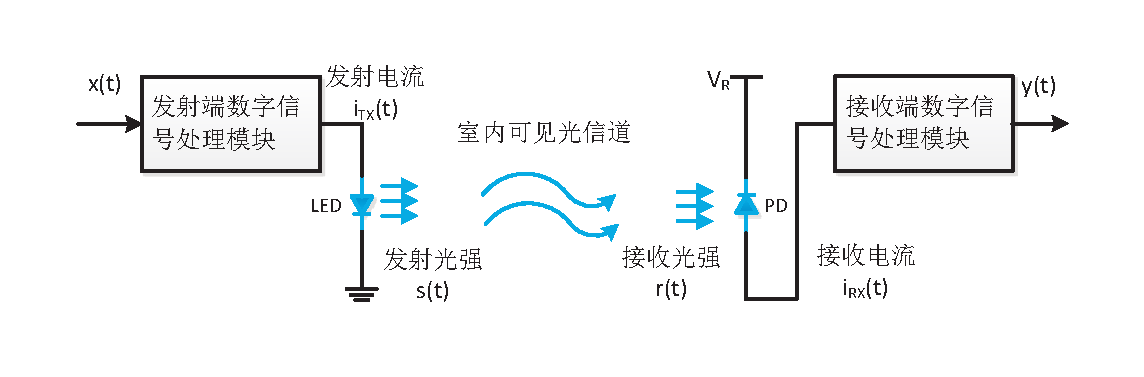
\includegraphics[width=\textwidth]{figures/chapter-2/BasicOpticalSystem.eps}
    \caption{光无线通信系统模型}
    \label{fig:BasicOpticalSystem}
\end{figure}
如\autoref{fig:BasicOpticalSystem}所示,在电信号域(Electrisity domain)发射端输出电压信号$x(t)$经过发光二极管后变成LED的电流$i_{TX}(t)$信号,接收端光敏二极管PD输出电流$i_{RX}(t)$,其最后转换成接收信号$y(t)$ ,在光信号域(Light Domain),首先在发射端发光二极管LED的电流信号$i_{TX}(t)$ 转变为发光强度$s(t)$,经过光信道后,在接收端光电二极管PD收到的光强信号为$r(t)$,经过光电转换,得到电流$i_{RX}(t)$。
所以在实际可见光通信系统中,信号传输由电光变换,光通道传输及光电变换三个过程组成,如\autoref{fig:BasebandModle}所示,接收端信号$y(t)$ 可以表示为:
\begin{equation}
    y(t)=x(t)\otimes h_1(t)\otimes h_2(t)\otimes h_3(t)+z(t)
\end{equation}
其中,$x(t)$表示发射端基带电压信号,$h_1(t)$表示电光转换系统的时域信道冲激响应(Channel Impose Response,CIR),$h_2(t)$表示可见光信道的时域信道冲激响应,$h_3(t)$表示光电转换系统的时域信道冲激响应
\cite{Yangxuecheng2015},
$z(t)$表示信道加性白高斯噪声(Additive White Gaussian Noise,AWGN),符从$z(t)\sim N(0,N_0/2)$分布,$N_0$为其功率谱密度,$\otimes$表示卷积运算。可见光通信系统的噪声,通常主要由热噪声和散弹噪声
\cite{Chenchunyan2014}。热噪声是一种高斯白噪声,在传统的射频无线通信系统中是很常见的。
散弹噪声也可以建模为白高斯噪声来处理,因为两个独立分布的高斯噪声还是高斯的,故我们可以将系统噪声统一建模为与信号独立的高斯白噪声。

\begin{figure}[htbp]
\centering
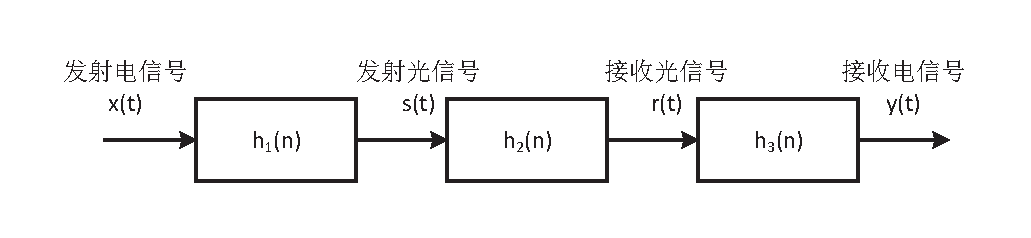
\includegraphics[width=0.9\textwidth]{figures/chapter-2/BasebandModle.eps}
\caption{光无线通信系统基带处理模型}
\label{fig:BasebandModle}
\end{figure}

\subsection{光电元器件简介}
如前文所述,可见光通信与传统的无线通信最大的区别在于调制与信号检测上,射频无线通信必须把基带信号通过调幅、调频或者调相技术调制到高频率的载波上,在接收端再下变频得到基带信号。但目前可见光通信器件技术还不能直接去调制光的幅度、频率或者相位,而是使用发射端强度调制和接收端直接检测技术。在发射端,需要电光转换器件将电信号转换成光信号,在室内可见光通信中用到的主要是发光二极管LED,LED就是调制器,其工作线性范围是一个非常重要的指标,因为如果输入信号的动态变化范围较大,超出LED的线性调制范围,则会发生非线性失真,将严重影响通信性能,在可见光OFDM系统中尤其要注意这点,另外,LED的响应时间是另一个重要指标,响应时间断的LED能够被更高频率的信号调制,也就意味着带宽增加、通信速率增高。在接收端,需要光电转换器件将光信号再变成电信号以进行解调解码,目前大量使用的是光电二极管PD,光电二极管的PN结面积相对比较大,以便接收更多的入射光,其在反向电压的作用下,没有光照时,反向电流非常小,称为暗电流;在有光照时,反向电流急速增大,并且在一定范围内反向电流功率与光照强度成正比。本节将详细介绍发光二极管和光电二极管的通信特性。
\subsubsection{电光转换器件}
目前在光通信领域使用得电光转换器件主要有激光二极管(Laser Diode,LD)和发光二极管LED两类,这两种器件的性质差异很大,应用场景也不同。激光二极管响应速度非常快,但是线性区间非常小,几乎只有关闭和激发两种状态,而且发光角度较小,通信时需要发射端与接收端对准,所以一般用于高速光纤通信中。这里我主要讨论室内无线光通信使用的发光二极管LED。

发光二极管LED是一种掺杂了镓(Ga)、砷(As)和磷(P)等化合物的半导体器件,它跟普通的二极管一样,具有单向导电性,内部有PN节,P区含有多余的电子,N区则有多余得空穴。当给发光二极管加正向电压时,P区的高能电子与N区的空穴结合发生能级跃迁变为低能电子,根据能量守能,其将向外辐射电磁波,并且包含波长在380 nm到780 nm之间的人眼可见的电磁波,具体辐射电磁波的波长主要由掺杂物的种类相关,这就是LED发光的基本原理。

\begin{figure}[htbp]
    \centering
    \subfloat[磷激发型LED光谱图]{
        \label{fig:OSTAR-Spectrum}
        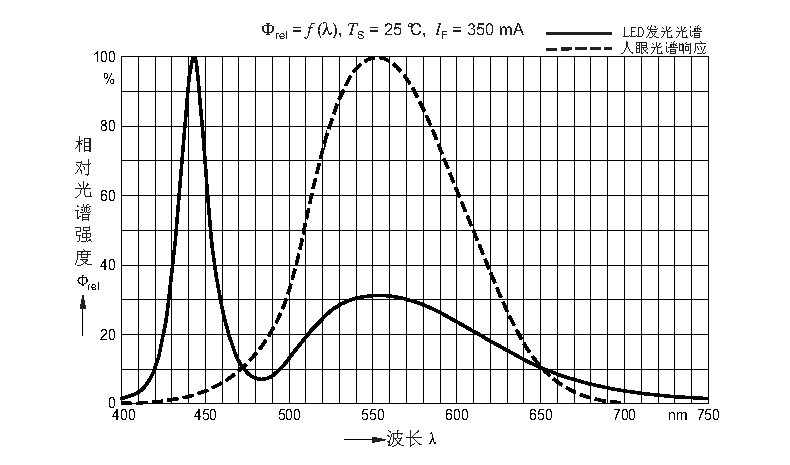
\includegraphics[width=0.5\textwidth]{figures/chapter-2/LEUWS2LN-RelativeSpectralEmission.eps}
    }
    \subfloat[RGB三原色混光型LED光谱图]{
        \label{fig:RGB-Spectrum}
        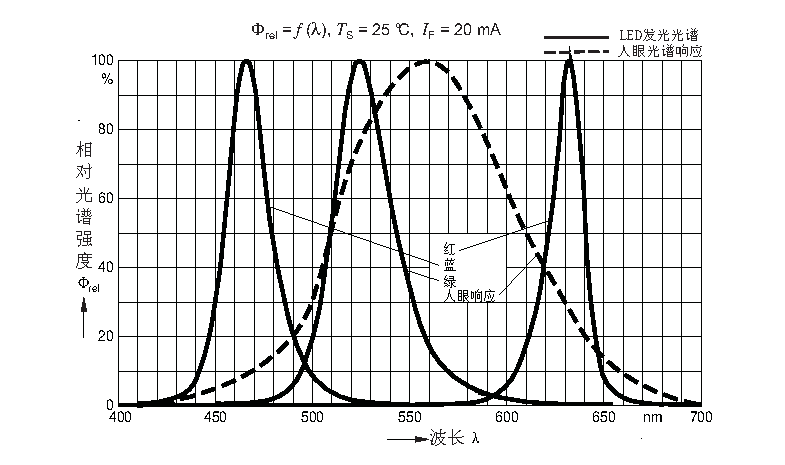
\includegraphics[width=0.5\textwidth]{figures/chapter-2/LRTBR98G-RGB-RelativeSpectralEmission.eps}
    }
    \caption{两种白色LED光谱对比图}
    \label{fig:WhiteLED}
\end{figure}

众所周知,白光是一种混合光,故我们日常用于照明的白光LED灯发出的白光也是由几种光合成的。现在市面上的白光LED主要有两种类型。一种是磷光激发型,由蓝光LED激发荧光物质发出黄光,然后蓝光与黄光混合成我们人眼看到的白光;另一种是多色混合型,由多个LED发出不同颜色的光直接合成为白光,这种类型常见的红绿蓝(RGB)LED灯内部就含有三块晶片,分别发红光、绿光和蓝光。图\ref{fig:OSTAR-Spectrum}所示是德国OSRAM公司生产的磷光激发型发光二极管Lighting Plus LE UM S2LN的相对光谱分布图\cite{LE2011},图中峰值位于445 nm处的是蓝光LED发出的蓝色光波,而峰值位于555 nm处的是蓝光激发荧光物质产生的黄光。因为激发荧光物质发黄光的响应时间过长,在使用磷光型LED进行可见光通信时,一般同时会在接收端加蓝色滤光片,滤掉响应过慢的黄光,所以虽然我们人眼看到的是白光,但是信号其实只调制在蓝光上,这就是前文中提到单色白光LED通信。图\ref{fig:RGB-Spectrum}所示多色混合型LED的相对光谱分布图\citep{LRTB2011},其具体型号为LRTB R98G,同为OSRAM生产。图中可见红绿蓝三种色光的峰值分别位于635 nm、525 nm和465 nm处,与林光激发型LED不同的是,红绿蓝三种色光分别由三种不同的LED晶片产生,都有很好的响应速度,我们可以对这三种色光分别调制,达到同时传输三路数据的目的,这样可以大大加大传输速率,即为前文所述的多色白光无线通信系统,也是本课题主要研究对象。


因为基于多色混合型LED的可见光通信系统能将各基色独立调制,总速率为各基色速率之和,所以相对于使用磷光激发型LED的单色光通信系统速率优势明显。现在也有专门的公司设计适合可见光通信的LED,如硅谷光擎(LED Engin),其生产了多种通信特性优异的多色混合型LED,如\autoref{fig:LED_LZ4_SputrcalPower}所示为型号为LZC-03MA07的多色混合型LED的相对光谱功率分布和绝对光谱功率分布。从图\ref{fig:LED_LZ4_relativeSputrcalPower}中可以看出各基色光之间隔离明显,相互之间的干扰很少,同时图\ref{fig:LED_LZ4_absoluteSputrcalPower}说明各基色的发光功率相差明显,在设计多色光通信系统时也可以优化各个基色光发射功率,减少干扰,这个是我们后面研究的内容。
\begin{figure}[h]
    \centering
    \subfloat[LZC-03MA07相对光谱功率分布]{
        \label{fig:LED_LZ4_relativeSputrcalPower}
        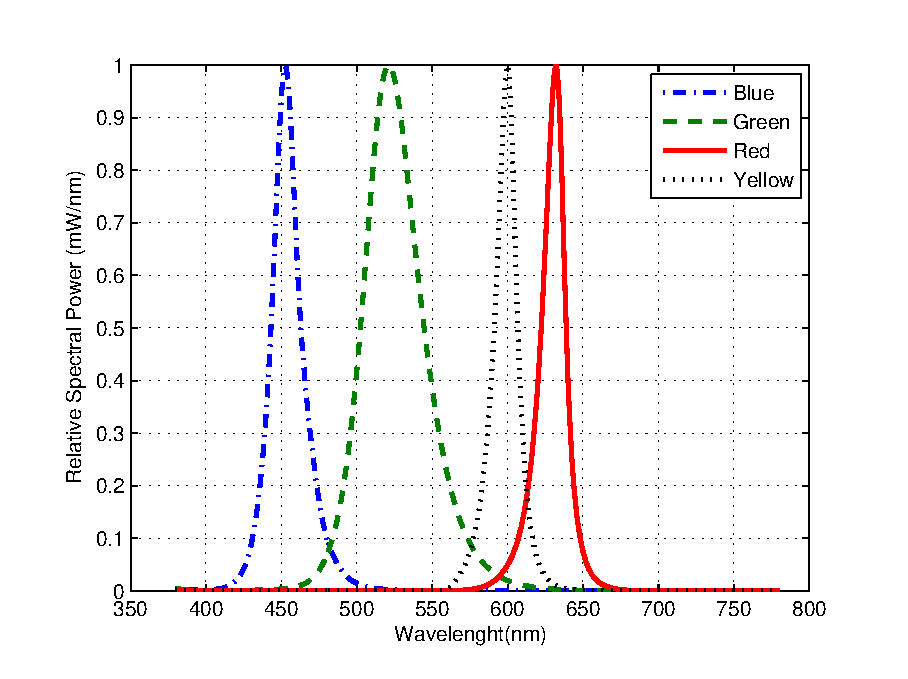
\includegraphics[width=0.5\textwidth]{figures/chapter-2/LED_LZ4_relativeSputrcalPower.eps}
    }
    \subfloat[LZC-03MA07绝对光谱功率分布]{
        \label{fig:LED_LZ4_absoluteSputrcalPower}
        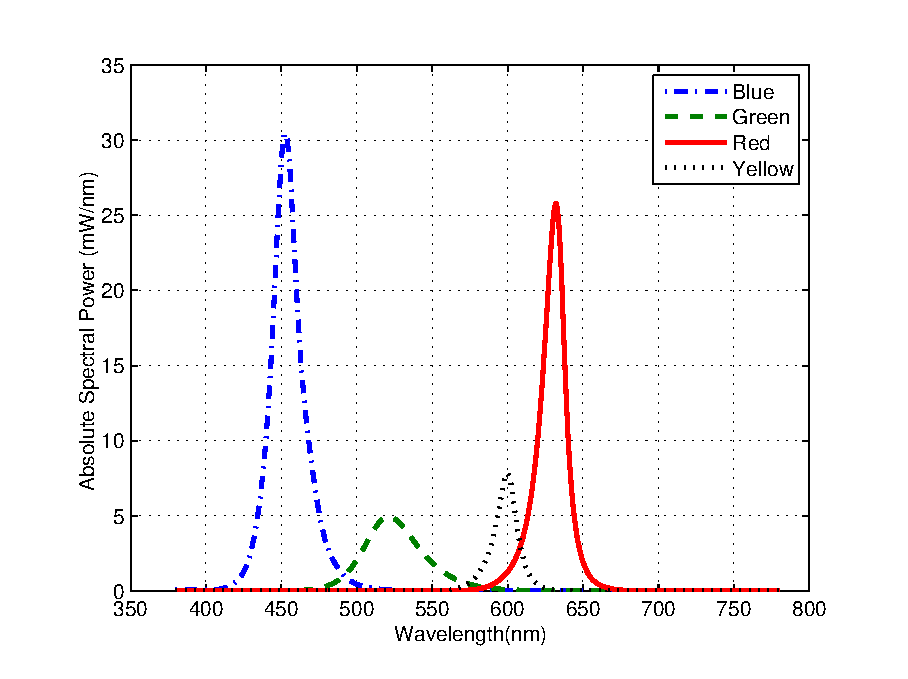
\includegraphics[width=0.5\textwidth]{figures/chapter-2/LED_LZ4_absoluteSputrcalPower.eps}
    }
    \caption{LZC-03MA07光谱功率分布}
    \label{fig:LED_LZ4_SputrcalPower}
\end{figure}
如前文所述,评价LED通信性能有两个重要的指标,一个是响应时间,另一个是线性区间长度,在多色混合型LED中,各基色LED的
\begin{figure}[ht]
\centering
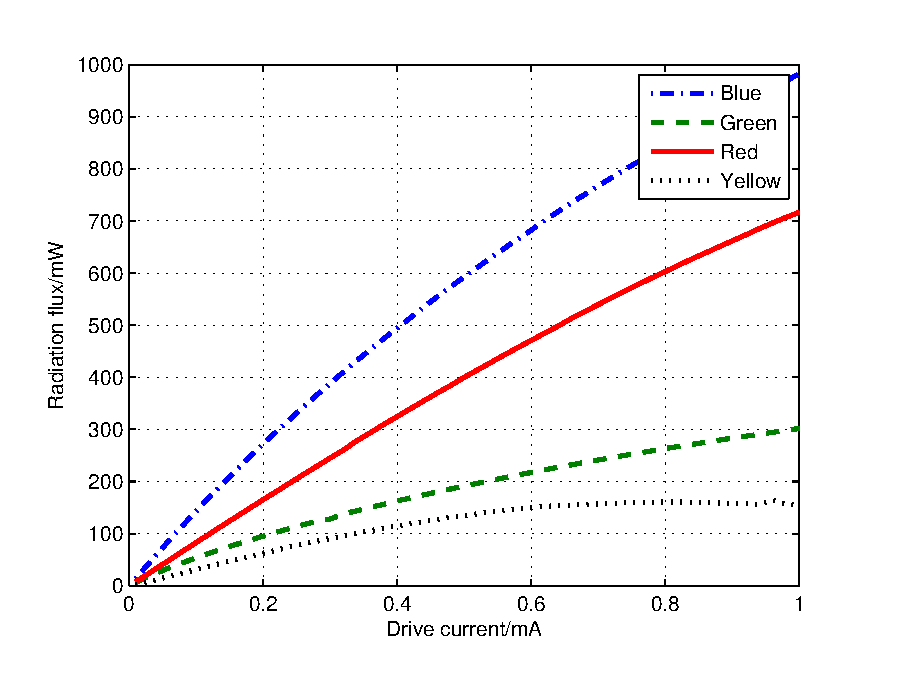
\includegraphics[width=0.8\textwidth]{figures/Chapter-2/LZ4radiationflux.eps}
\caption{LZC-03MA07的辐射通量随驱动电流的变化曲线}
\label{fig:LZ4radiationflux}
\end{figure}
\section{OFDM技术在室内可见光通信中的应用}
\subsection{OFDM技术简介}
\subsection{可见光中的OFDM调制}
\section{自适应传输技术简介}
\section{本章小结}

   %% !Mode:: "TeX:UTF-8"
\chapter{可见光多波段OFDM系统的信道估计}
\section{引言}
所谓信道估计,就是在接收端估计出信道状态信息(Channel State Information,CSI),为下一步地解调做准备,也是自适应传输技术的基础。无线通信一个重要的特征就是发射端到接收端之间的路径比较复杂,不像有线通信那样是固定且可预知的,所以信道估计技术在无线通信领域格外重要,特别是在OFDM 等需要相干检测的系统中。本章将着重介绍信道估计技术,首先介绍传统射频通信中OFDM 系统的信道估计方法,然后具体到可见光通信系统中的信道估计问题,再将结合实际系统设计,讨论信道的非线性问题,最后将研究多色可见光通信系统中各波段之间串扰的估计。
\section{OFDM信道估计常用方法}
信道估计总体可以分为两大类,盲信道估计和基于导频的信道估计。盲信道不需要额外的导频或者训练序列,因此频率利用率高;但是它的缺点是计算量大、算法复杂,而且精度低、收敛速度缓慢,难以用于移动通信环境
\cite{石钧2012ofdm}。基于导频的信道估计原理是在发射端插入专门用于信道估计的导频或者训练序列,并且这些序列对于接收端也是已知的,接收端根据接收到的经过了信道后的导频序列与原导频序列之间的关系,估计出信道冲击响应(Channel Impulse Response,CIR)。这类信道估计方法因为要插入导频序列会稍微降低整个系统的传输速率,但是其估计实现复杂度低、估计精度高,在实际工具中大都采用这种方法。本节也主要讨论基于导频的信道估计算法。
\begin{figure}[htbp]
    \centering
    \subfloat[块状导频放置方式]{
        \label{fig:BlockTypePilot}
        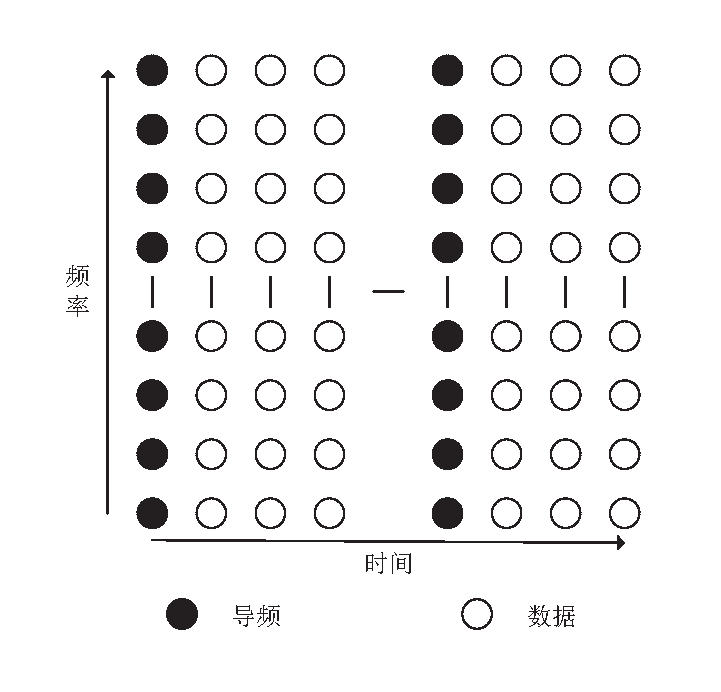
\includegraphics[width = 0.5\textwidth]{figures/Chapter-3/BlockTypePilot.eps}
    }
    \subfloat[梳状导频放置方式]{
        \label{fig:CombTypePilot}
        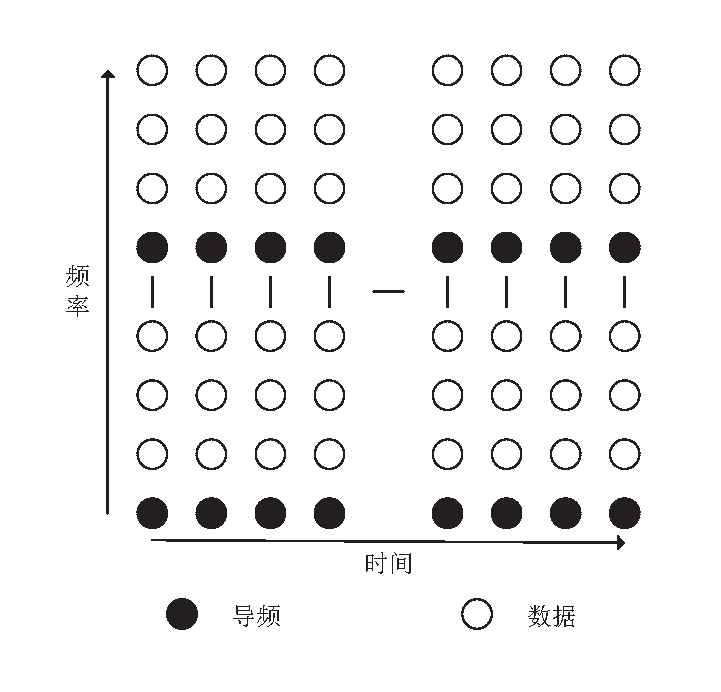
\includegraphics[width = 0.5\textwidth]{figures/Chapter-3/CombTypePilot.eps}
    }
    \caption{导频放置方式}
    \label{fig:PilotAllocation}
\end{figure}






\section{可见光信道估计}
\section{可见光信道非线性分析}
\section{可见光各波段之间串扰估计}
\section{本章小结}

  %  % !Mode:: "TeX:UTF-8"
\chapter{可见光多波段OFDM系统速率自适应技术研究}
\section{引言}
自适应传输技术在上世纪60年代就已经被提出,其基本思想就是根据实时的信道质量决定调制参数,目标是优化通信质量,但是因为其计算复杂度很大,实现困难而没有引起研究人员足够的重视\cite{徐凌峰2007ofdm},直到上世纪80年代末,人们对高速可靠的通信系统的需求越来越强烈,同时由于数字集成电路的快速发展,其计算能力已能够支撑复杂的算法,所以自适应传输计算重新进入研究人员的视野,并且成功用于DSL、WCDMA等通信系统。前面我们已经介绍过OFDM系统及其信道估计的方法,已经了解OFDM技术是把实际通信信道划分成若干个子信道,每个子信道可以认为是独立传输的,如果所有的子载波上都使用同样的调制方式,那么整个系统的误比特率性能就由那些处于深衰落处的子载波决定,如在前两章已经介绍室内可见光信道就是低通的,则此时高频的子载波决定了整个系统的性能,这样的方法显然是不合理的,所以在第三章的仿真中就使用了表\ref{tab:modOrder}所示的调制策略,但是之前得到这样的策略是由主观判断得到的,而没有充足的理论依据。本章将详细介绍OFDM自适应技术及其在可见光通信中的应用,首先将从信息论的角度探讨自适应传输的原理,然后将介绍现有的几种经典的自适应算法并且仿真分析它们的性能,最后将介绍一种可见光自适应传输方案。
\section{自适应传输的信息论基础}
通信技术经过将近一个世纪的发展,不断出现的使得系统传输速率越来越高,因此人们要问在特定的通信信道下传输速率的极限是什么?这正是经典的香农信息论已经回答的问题,同时也给系统设计者指明了要达到这个极限系统要满足的条件,虽然这些严苛的条件在实际设计中不可能完全满足,但是已有很多系统的系统已经很接近香农限了。

自适应传输是一种提高频谱利用率的通信技术,同样也满足香农信息论关于信道容量的结论,所以自适应传输技术也不可能使得实际系统传输速率突破香农限,而是在香农信息论的指导下去设计系统,使得系统逼近这一极限,因此在讨论自适应传输的具体算法之前了解一些香农信息论的知识非常必要。
\subsection{高斯信道容量}
信道容量是一个通信信道环境一个重要的度量指标,它的含义是在该信道下传输速率的上限,如果本身信道容量就很小的环境下,无论使用何种通信技术也不能实现高速通信系统,反之在信道容量大的信道环境下,可以通过精心设计系统以达到高速通信的目的。在香农信息论中,信道容量是用互信息量来描述的,其数学表达式为:
\begin{equation}
C = \arg \underset{P_x(X)}{\text{max}} \ I(X;Y)
\end{equation}

\begin{equation}
I(X;Y)=\sum_{x,y}p(x,y)\log_2\frac{p(x,y)}{p(x)p(y)}
\end{equation}
式中$I(X;Y)$表示发送信号X与接收信号Y之间的互信息,p(x)、p(y)和p(x,y)分别表示X=x的概率,Y=y的概率及X=x并且Y=y的联合概率。根据上面的定义,我们可以得到在高斯信道下的信道容量公式为:
\begin{equation}
C = B\log_2\left(1+\frac{S}{N_0B}\right)=B\log_2(1+\gamma)
\end{equation}
上式中B为高斯信道带宽,S为输入信号的平均功率,$N_0$为单边带高斯噪声功率谱密度,$\gamma=\frac{S}{N_0B}$表示接收信噪比。该容量是当发送信号X服从高斯分布时取得。而在实际的数字传输系统中,这个条件是无法满足的,所以该信道容量只能作为系统传输速率的上限。
\subsection{注水定理}
在无线通信环境下,由于放大器等硬件是非理想的,并且信号在传输过程中会发生散射、反射等造成多径,实际的通信系统信道远比加性高斯信道复杂得多。我们假设信道的传输函数为$H(f)$,输入信号的功率谱密度为$S(f)$,单边带高斯噪声功率密度还是$N_0$。为了推导这样的信道的信道容量,可见将整个信道带宽均分为N个子信道,则每个子信道的带宽为$B/N$,当N足够大时,中心频率为$f_i$处的子信道可以看作是信道增益为$H(f_i)$的带限信道。于是整个信道容量等于所以子信道容量之和:
\begin{equation}
\begin{aligned}
C&=\lim_{N\rightarrow \infty}\sum_{i=1}^{N}\Delta f\log_2\left(1+\frac{S(f)|H(f)|^2\Delta f}{N_0 \Delta f}\right) \\
&=\int_B \log_2\left(1+\frac{S(f)|H(f)|^2}{N_0}\right)df
\end{aligned}
\end{equation}
从上式中可以看出信道传输函数H(f)和发送信号的功率谱密度分布及噪声功率共同决定了信道容量的大小。假设系统发射功率受限,即:
\begin{equation}
\label{equ:powerLimit}
\int_B S(f)df=P
\end{equation}
则由拉格朗日乘子法计算可得,当S(f)的分布满足下式时可以达到信道容量。
\begin{equation}
\label{equ:water_filling}
S(f)=
\begin{aligned}
\begin{cases}
K-\frac{N_0}{|H(f)|^2},&\ |H(f)|^2\geq\frac{N_0}{K} \\
0  ,&\ |H(f)|^2<\frac{N_0}{K}
\end{cases}
\end{aligned}
\end{equation}
其中K为常数,并且满足式\ref{equ:powerLimit}中的功率受限条件。

式\ref{equ:water_filling}得到S(f)分布的过程也称为“注水定理”或者“注水算法”,它表示要想在传输函数为H(f),噪声功率密度为$N_0$的信道下要达到信道容量S(f)的分布一定要满足上式。其物理含义是:当信噪比$|H(f)|^2/N_0$较大时,应该给该处的子信道分配更多的功率;反之当信噪比很小时,分配的功率也很小;甚至当信噪比过小(小于1/K)时不分配功率。
\begin{figure}[htbp]
\centering
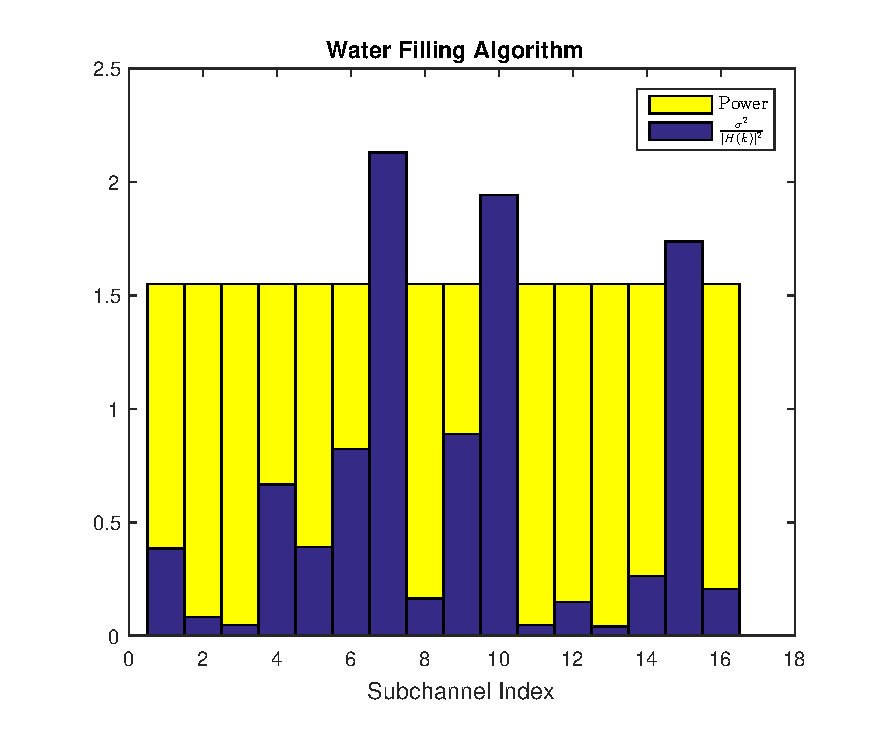
\includegraphics[width=0.8\textwidth]{figures/chapter-4/waterFilling.eps}
\caption{注水定理示意图}
\label{fig:waterFilling}
\end{figure}
OFDM技术的基本原理就是将整个信道划分为相互正交的并行子信道,这个与前面注水算法的推导过程很相识,只是OFDM系统中子载波的数目是有限的,调制阶数是离散的。从此可以看出注水算法很容易在OFDM系统中现实,我们将在下一节中详细介绍。
\section{OFDM系统自适应算法研究}
在一个有N个子载波的OFDM系统中,假设各个子载波上的信道增益$h_k=|H(k)|^2(k=0,1,\cdots,N-1)$和高斯噪声方差$\sigma^2$已知,若$b_k$ 和$p_k$分别表示分配到第k 个子载波上比特数和功率,如设置误比特率为固定值$\text{BER}_{target}$,则香农公式$b_k$与$p_k$有如下关系:
\begin{equation}
b_k = \log_2(1+\frac{h_kp_k}{\Gamma\sigma^2})
\end{equation}
也可以写为:
\begin{equation}
p_k = \frac{\Gamma\sigma^2}{h_k}(2^{b_k}-1)
\end{equation}
其中$\Gamma$表示信噪比差(SNR gap),它由误比特率BER及调制星座图决定,对于QAM调制,如不加信道编码,则$\Gamma$与$\text{BER}_{target}$之间关系如下\cite{余官定2005ofdm}:
\begin{equation}
\Gamma = -\frac{\ln(5\cdot\text{BER}_{target})}{1.5}
\end{equation}

OFDM自适应传输在不考虑信道编码的情况下其实就是比特和功率在各个子载波上分配问题,它可以有传输速率、发射功率和误比特率三个优化目标量,这样也就有三种优化准则,即固定误比特率和功率的速率最大化(Rate Adaptive,RA)准则、固定误比特率和速率的功率最小化(Margin Adaptive, MA)准则和固定功率与速率的误比特率最小化(BER Adaptive, BA)准则。同时需要提出的是,与前面的理论分析不同,实际系统可以选择的调制方式是离散的($b_k \in \mathbb{N}$,$\mathbb{N}$表示整数集),也就是说OFDM自适应其实是一个整数优化问题(Integer Programming,IP),之前在推导注水算法时用到的拉格朗日乘子法不能再用到实际系统中,需要根据实际系统的需要,根据优化准则去选择合适的优化方法,下面将介绍几种经典的OFDM自适应算法。
\subsection{Hughes-Hartogs算法}
Hughes-Hartogs算法\cite{hughes1989ensemble}受数学中“贪婪(Greedy)优化”的启发,本质上也是一种贪婪算法,由Hughes-Hartogs于1988年提出,其描述如下:假设OFDM系统中各个子载波上的信道增益和噪声都是已知的,这样在特定的BER要求下要传输1比特所需要的功率也是可知的,Hughes-Hartogs算法就是每次遍历一次所有的子载波,选择需要功率最少的子载波放置1比特数据,如此循环迭代,知道用完所有功率(RA准则)或者达到目标速率(MA准则)。对于RA 准则和MA准则,Hughes-Hartogs算法是最优的。它的具体实现步骤如下:
\begin{description}
\item{\bf{步骤1:}}令$b_k(k=0,1,\cdots,N-1)$,$P=\sum_{i=0}^{N-1}p_k=0$,$R=\sum_{i=0}^{N-1}b_k=0$,$P$表示已用的功率,$R$表示已分配比特。
\item{\bf{步骤2:}}遍历计算每个子载波上增加1比特所需要增加的功率:
\begin{equation}
\Delta p_k=\frac{\Gamma\sigma^2}{h_k}(2^{b_k+1}-1)-\frac{\Gamma\sigma^2}{h_k}(2^{b_k}-1)=\frac{\Gamma\sigma^2}{h_k}2^{b_k}
\end{equation}
\item{\bf{步骤3:}}找到所需增加额外功率的子载波:
\begin{equation}
k^{\star} = \arg\ \underset{0\leq k \leq N-1}{\min}\Delta p_k
\end{equation}
对于RA准则,若$P+\Delta p_{k^\star}\geq P_{total}$则结束算法,反之则置$b_{k^\star}=b_{k^\star}+1$,$P=P+\Delta p_{k^\star}$,返回\textbf{步骤2}继续执行;对于MA准则,若$P+\Delta p_{k^\star}\geq P_{total}$或者$R+1\geq R_{target}$则结束算法,反之则置$b_{k^\star}=b_{k^\star}+1$,$P=P+\Delta p_{k^\star}$,$R=R+1$返回\textbf{步骤2} 继续执行。其中$P_{total}, R_{target}$表示限制功率和目标速率。
\end{description}
该算法的得到的最后结果为$b_k, k=0,1,\cdots,N-1$即为每个子载波上应该分配的比特数,如果$b_k=0$则说明该子载波处信道质量太差,应设置为虚拟子载波不传输数据。从算法的步骤中可以看出每次迭代找到的都是最优的子载波,所以整个算法也是最优的,但是其复杂度为$O(R\cdot N)$,对于RA准则而言,随着信噪比的增加,可传输速率$R$也会增大,Hughes-Hartogs算法复杂度也会增加,同时子载波数的增加也会增加算法的复杂度,这也限制了Hughes-Hartogs算法在工程中的应用。
\subsection{P.S.Chow算法}
P.S.Chow算法\cite{chow1995practical}是一种RA准则下次优算法,即限定了发射功率和速率优化误比特率性能。它由P.S.Chow于1995年提出,该算法总体上分三步进行,第一步迭代找到(近似)最优系统性能门限$\gamma_{margin}(dB)$ (该门限表示系统在能够达到目标误比特率基础上还能容忍的额外噪声,以dB为单位);第二步确定各个子载波上的比特分配,如果第一步迭代在迭代次数达到上限后还没有收敛,即$R\neq R_{target}$,则会在这步调整使得$R=R_{target}$;第三步是功率分配,首先根据根据各个子载波上的比特数和目标误比特率得到各个子载波上所需功率,然后总功率也限制功率之间的关系,得到一个功率系数,调整各个子载波上的功率,使得总功率满足功率限制。具体算法步骤如下:
\begin{description}
\item{\bf{步骤1:}}计算各个子载波上的信噪比$SNR(k),\forall k$,并且假设各个子载波上是归一化等功率的,即$p_k=1, \forall k$。
\item{\bf{步骤2:}}令$\gamma_{margin}=0 (dB), IterateCount =0$和$UsedCarriers=N$,其中$IterateCount$表示迭代计数器,$UsedCarriers$表示使用的子载波。
\item{\bf{步骤3:}}根据下面的式子,遍历所有子载波计算$b(k),\hat{b}(k),diff(k)$:
\begin{eqnarray}
b(k)=\log2(1+\frac{SNR(k)}{\Gamma+\gamma_{margin}(dB)})\\
\hat{b}(k)=round[b(k)]\\
diff(k)=b(k)-\hat{b}(k)
\end{eqnarray}
$round[\cdot]$表示取整,如果$\hat{b}(k)=0$,则$UsedCarriers=UsedCarriers-1$。
\item{\bf{步骤4:}}令$R=\sum_{k=0}^{N-1}\hat{b}(k)$,若$R=0$说明整个信道条件太差,无法传输数据,算法退出。
\item{\bf{步骤5:}}用下式更新$\gamma_{margin}$:
\begin{equation}
\gamma_{margin}=\gamma_{margin}+10\log_{10}(2^{\frac{R-R_{target}}{UsedCarriers}})
\end{equation}
其中$R_{target}$表示目标速率。
\item{\bf{步骤6:}}令迭代计数器加1,$IterateCount=IterateCount+1$。
\item{\bf{步骤7:}}若$R\neq R_{target}$ 并且 $IterateCount<MaxCount$,则令$UsedCarriers=N$跳到\textbf{步骤3} 执行,否则跳到\textbf{步骤8}。其中$MaxCount$表示设置的最大迭代次数。
\item{\bf{步骤8:}}若$R>R_{target}$,则选择:
\begin{equation}
k^{\star} =\arg\ \underset{0\leq k\leq N-1}{\min}diff(k)
\end{equation}
令$\hat{b}(k^{\star})=\hat{b}(k^{\star})-1$,$diff(k^{\star})=diff(k^{\star})+1$,重复执行\textbf{步骤8}直到$R=R_{target}$
\item{\bf{步骤9:}}若$R<R_{target}$,则选择:
\begin{equation}
k^{\star} =\arg\ \underset{0\leq k\leq N-1}{\max}diff(k)
\end{equation}
令$\hat{b}(k^{\star})=\hat{b}(k^{\star})+1$,$diff(k^{\star})=diff(k^{\star})-1$,重复执行\textbf{步骤9}直到$R=R_{target}$
\item{\bf{步骤10:}}根据前面得到各子载波上分配的比特$\hat{b}(k), k=0,1,\cdots,N-1$,计算各个子载波上应该分配的功率$p_k$使得各个子载波上的误比特率$P_e(k)=P_{e,target}, \forall k$成立。这样就会改变了步骤1中的等功率分配了。
\item{\bf{步骤11:}}在步骤10中得到的各个子载波上的功率基础上再乘以一个比例因子,使得发射总功率$P=\sum_{k=0}^{N-1}p_k=P_{total}$,$P_{total}$表示额定功率。
\end{description}

P.S.Chow 算法的思想是先通过目标速率$\text{Rate}_{target}$迭代寻找最优系统性能门限$\gamma_{margin}$,迭代终止条件为分配的总速率等于目标速率,但是在某些信道条件下,总速率会在目标速率附近震荡而永远不会收敛到目标速率,因此Chow算法还设计了另一个收敛条件,即迭代次数$IterateCount$等于初始化设置的最大迭代次数$MaxCount$。如果是由迭代次数限制而终止迭代的,则通过步骤8、9来保证总速率等于目标速率,得到各个子载波上的比特分配,然后根据各子载波上的比特分配确定各个子载波上需要的功率,最后在各个子载波的功率前面乘以一个相同的系数,使得总功率满足功率限制条件,其最坏情况下算法复杂度为$O(MaxCount\cdot N+2N)$,一般情况下$MaxCount$小于10 次就会收敛,所以相对于Hughes-Hartogs算法,其算法复杂度下降了很多。
\subsection{Fischer算法}
Fischer算法\cite{fischer1996new}也是一种固定发射功率和速率优化系统误比特率的算法(RA准则),但是它与Hughes-Hartogs算法和P.S.Chow算法不同,这两者都是从信道容量的角度出发的,而Fischer算法则是从各个子载波上的误比特率出发,算法的核心思想认为当所有被利用的子载波上的误符号率相等时,则会使得系统的误比特率最优,这个其实也比较容易理解,因为如果有某些子载波的误符号率很高的话,则这些子载波就决定了整个系统的误比特率。

Fischer是根据QAM调制的误符号率来推导的,第$k$各子载波上的误符号率$P_s(k)$可以写为:
\begin{equation}
P_s(k)=4\cdot Q\left(\sqrt{\frac{d_k^2/4}{\sigma^2_k/2}}\right)
\end{equation}
其中$Q(x)=1/\sqrt{2\pi}\int_x^{\infty}exp\{-t^2/2\}dt$是互补高斯积分函数,$d_k, \sigma^2_k$分别表示第$k$个子载波上调制星座图中的最小欧氏距离和噪声方差。要使得使得所有子载波上的误符号率都相等,也就是使得归一化信噪比$SNR_0$等于一个常数,即:
\begin{equation}
SNR_0 = \frac{d_k^2/4}{\sigma^2_k/2}=const
\end{equation}
整个优化问题就是在功率和速率的限制下最大化$SNR_0$。又因QAM调制的符号可以表示为$V_k\cdot\{(\pm 1,\pm3,\cdots)+j(\pm 1,\pm3,\cdots)\}$,$V_i$表示增益系数,则有$d_k^2=4V_k^2$,并且第$k$个子载波上的平均功率为:
\begin{equation}
\label{equ:power_equal}
p_k = V_k^2\cdot \frac{2}{3}2^{b_i} = SNR_0\frac{\sigma^2_k}{2}\frac{2}{3}2^{b_k}
\end{equation}
$b_k$表示第$k$个子载波上放置的比特数,利用功率限制条件有:
\begin{equation}
P_{total} = \sum_{k=0}^{N-1}p_k=\frac{SNR_0}{3}\sum_{k=0}^{N-1}\sigma_k^2\cdot 2^{b_k}
\end{equation}
所以有:
\begin{equation}
SNR_0 = \frac{3P_{total}}{\sum_{k=0}^{N-1}\sigma^2_k\cdot 2^{b_k}}
\end{equation}
要最大化$SNR_0$,在功率和速率限制条件下,利用拉格朗日优化得到$\sigma_k^2\cdot 2^{b_k}, k = 0,1,\cdots N-1$为常数,利用这个结有:
\begin{equation}
(\sigma_k^2\cdot 2^{b_k})^N = \prod_{i=0}^{N-1}\sigma_i^2\cdot 2^{b_i} = 2^{R_{target}}\cdot \prod_{i=0}^{N-1}\sigma_i^2
\end{equation}
因为$\sigma_k^2\cdot 2^{b_k}, \forall k$都相等,所以得到:
\begin{equation}
b_k = \frac{R_{target}}{N} +\frac{1}{N}\log_2\left(\frac{\prod_{i=0}^{N-1}\sigma_i^2}{\sigma_k^{2N}}\right)
\end{equation}
通过上式得到各个子载波上的比特分配之后,要在可用子载波集合$\mathrm{I}$ 中去掉$b_k\leq 0$的子载波,并且更新可用的子载波数为$N^{\prime}$,利用上式迭代,直到$b_k>0, \forall k\in \mathrm{I}$。因为$\sigma_k^2\cdot 2^{b_k}$为常数,由式\ref{equ:power_equal}可知所有可用的子载波上的能量也应该相等:
\begin{equation}
p_k = \frac{P_{total}}{N^\prime}, \forall k \in \mathrm{I}
\end{equation}

上面只是理论上的推导,没有限制$b_k$为整数,但是在实际应用中必须要加上这一条件,相应的算法也有小许改动,下面给出Fischer算法的具体实现步骤:
\begin{description}
\item{\bf{步骤1:}}首先计算各子载波上的等效噪声方差(等于实际噪声方差除以信道增益)$\sigma_k^2,k=0,1,\cdots,N-1$,$N$为子载波数。然后计算各子载波上的对数噪声$LDN_k=\log_2(\sigma_k^2),k=0,1,\cdots,N-1$,将这些值保存下来,之后的计算中可以重复使用;初始化$\mathrm{I}=\{0,1,\cdots,N-1\}$,$N^\prime=N$。
\item{\bf{步骤2:}}计算可用的子载波上应该分配的比特数:
\begin{equation}
b(k) = \frac{R_{target}+\sum_{i\in \mathrm{I}}LDN_i}{N^\prime}-LDN_k
\end{equation}
\item{\bf{步骤3:}}在集合$\mathrm{I}$中去掉所有$b(k)\leq 0$的$k$,并且更新$N^\prime$,跳转到\textbf{步骤2}执行,直到$b(k)>0, \forall k\in \mathrm{I}$。
\item{\bf{步骤4:}}量化分配的比特,$\hat{b}(k)=round(b(k))$,记录量化误差$diff(k)=b(k)-\hat{b}(k)$。
\item{\bf{步骤5:}}计算总比特数$R=\sum_{k\in \mathrm{i}}\hat{b}(k)$
\item{\bf{步骤6:}}若$R=R_{target}$,则跳转到\textbf{步骤7},否则:\\
若$R>R_{target}$,则选择量化误差最小的子载波,假设其序号为$k^\star$,调整$\hat{b}(k^\star)=\hat{b}(k^\star)-1$,$R=R-1$,$diff(k^\star)=diff(k^\star)+1$,继续步骤6直到$R=R_{target}$;\\
若$R<R_{target}$,则选择量化误差最大的子载波,假设其序号为$k^\star$,调整$\hat{b}(k^\star)=\hat{b}(k^\star)+1$,$R=R+1$,$diff(k^\star)=diff(k^\star)-1$,继续步骤6直到$R=R_{target}$;
\item{\bf{步骤7:}}最后根据各个子载波上分配的比特数,按下式计算各子载波上应该分配的功率:
\begin{equation}
p_k = \frac{P_{total}\cdot \sigma_k^2\cdot 2^{\hat{b}(k)}}{\sum_{i\in \mathrm{I}}\sigma_i^2\cdot 2^{\hat{b}(i)}}
\end{equation}
\end{description}

Fischer算法给出了比特和功率分配的闭式解(经有限次迭代之后一定收敛),而且算法复杂度比较低,通过在步骤1中把$LDN_k, k=0,1,\cdots,N-1$存储下来,在接下来的运算中只需要进行加减法和除法运算,尤其是当目标速率设置适当(步骤5中计算得到的$R$接近$R_{target}$)时,算法复杂度可以进一步降低,为$O(N)$量级,相对于P.S.Chow算法又有了降低。

上面介绍了三种非常经典的OFDM系统比特功率分配算法,也有研究人员对这些算法进行改良,如改进的贪婪算法不像原算法逐比特分配,而是先通过对分法搜索得到注水定理中的注水线(注水线的上下界是确定的\cite{余官定2005ofdm}),然后根据注水线得到各子载波上的比特数并向下取整,计算这些比特所需要的功率,最后用贪婪算法剩下的功率。这种改进的算法在高信噪比下可以大大降低复杂度。也有学者通过迭代的方式将注水算法应用到离散比特分配中,其基本思路是先令注水线等于其上界,然后按这个注水线分配比特并且四舍五入取整并计算所需的功率,如果功率满足限制条件则分配完毕,否则降低注水线重新注水,直到满足功率限制。

\subsection{仿真结果分析}
\begin{figure}[htbp]
\centering
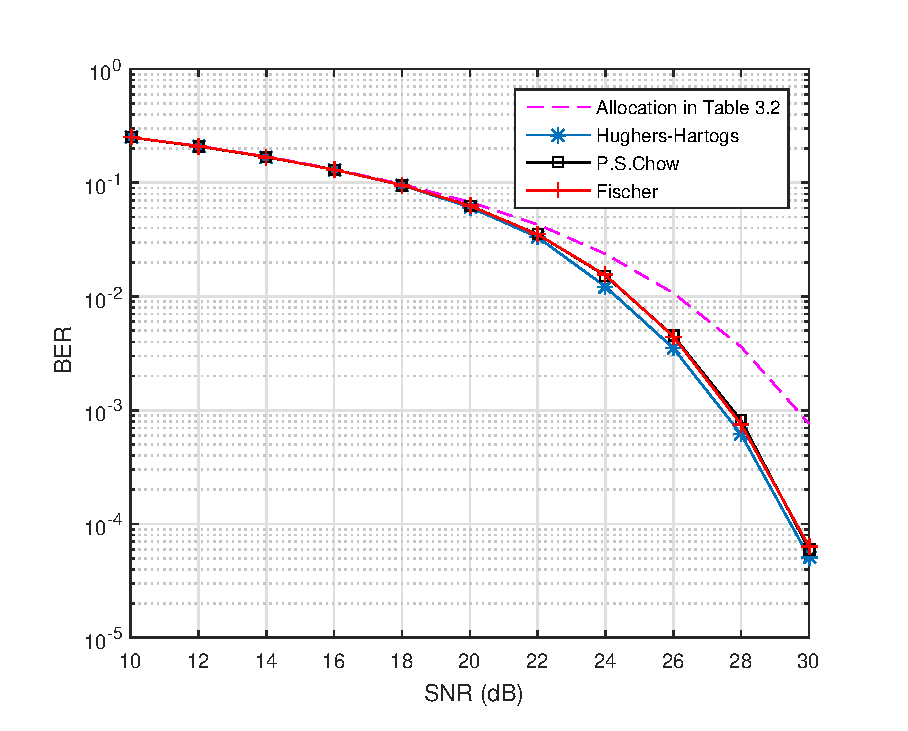
\includegraphics[width=0.8\textwidth]{figures/chapter-4/BERonDiffAlgo.eps}
\caption{LOS信道下不同比特功率算法误比特率性能比较}
\label{fig:berOnDiffAlgo}
\end{figure}

\begin{figure}[htbp]
\centering
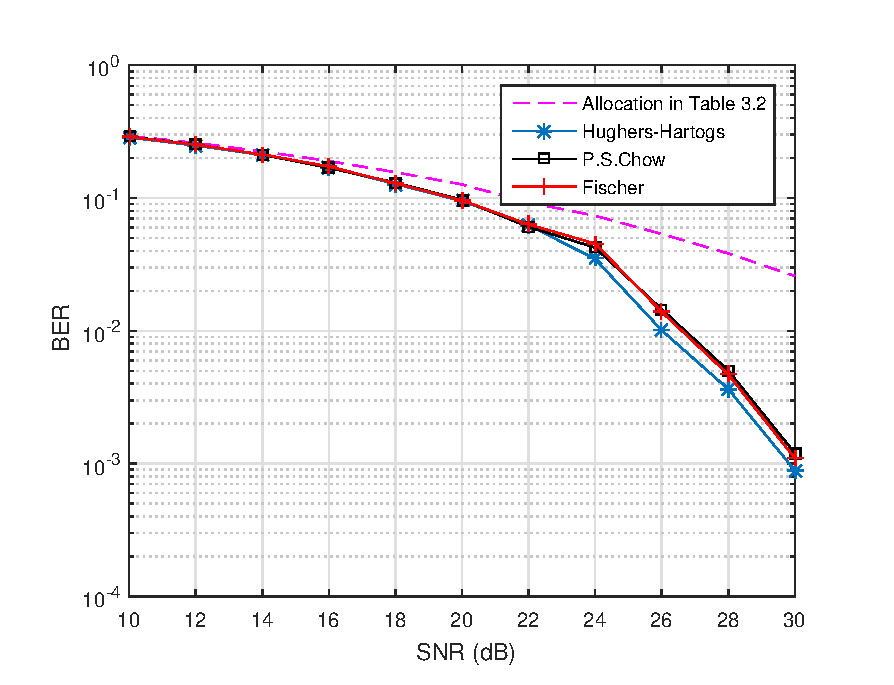
\includegraphics[width=0.8\textwidth]{figures/chapter-4/DOWBERonDiffAlgo.eps}
\caption{DOW信道下不同比特功率算法误比特率性能比较}
\label{fig:DOWBERonDiffAlgo}
\end{figure}
前面介绍了三种不同的比特功率分配算法,下面通过仿真来展示其性能。仿真的信道还是使用\ref{subsection:Channel}节中的可见光LOS信道和DOW信道,使用LOS信道更贴近本课题的硬件设计,而使用DOW信道模型可以增加信道的多样性,更能客观地比较不同算法之间的性能差别。仿真中使用QAM调制,并且在仿真中对最高调制阶数进行了限制(1024QAM),这个在实际工程中也是常见的,毕竟很少有系统用到1024QAM以上的调制。

图\ref{fig:berOnDiffAlgo}给出了在LOS信道不同比特功率分配算法的误比特率随信噪比变化的性能,为了便于比较,将目标速率$\text{Rate}_{target}$设置为736 bit/OFDM signal,与表\ref{tab:modOrder}中的相等。图中可以看出,虽然在表\ref{tab:modOrder}中我们已经专门针对可见光通信的低通特意设计了比特分配,但是使用自适应算法得到比特功率分配在性能上还是有些提高的,尤其是在高信噪比的情况下。但是在固定的LOS信道下,Hughes-Hartogs算法、Chow算法和Fischer算法之间的BER性能差异很小,这也说明了Chow算法和Fischer算法在计算复杂度降低的情况下,性能损失不大。需要说明的是,Hughes-Hartogs算法在RA和MA准则下是最优的,但是这里BER 性能的比较是BA准则,Hughes-Hartogs算法在BA准则下的计算过程是先使用MA准则得到各子载波的分配的比特,然后根据计算每个子载波达到目标BER所需要的功率,最后归一化使得总功率满足功率限制,所以在BA准则下Hughes-Hartogs算法也不是最优的。图\ref{fig:DOWBERonDiffAlgo}展示了各种比特功率分配算法在DOW信道模型下的性能,这里DOW信道模型采用的是\ref{subsection:Channel}节中提到的指数衰减模型和天花板反射模型混合得到信道模型,结果也LOS信道下类似,三种算法BER性能都优于表3.2 中的分配方案,但是三种算法之间的性能非常接近。

图\ref{fig:loadedBit}和\ref{fig:loadedPower}给出了三种算法在各个子载波上分配的比特和功率,可以看出分配的比特数随着频率(子载波系数)的增加而减少,这是因为我们的信道是低通的,给低频段高信噪比的子载波分配更多比特而在高频段低信噪比的子载波分配更少比特是合理的。各子载波上分配的功率上下波动,但是有个规律- 在分配了相同比特的子载波上,功率是随着频率递增的,这还是由于低通信道,在相同阶数的调制的子载波上为了使得BER尽可能相等,高频的子载波要分配更多的比特。综上所述仿真结果是与之前的理论分析相吻合的。
\begin{figure}[htbp]
\centering
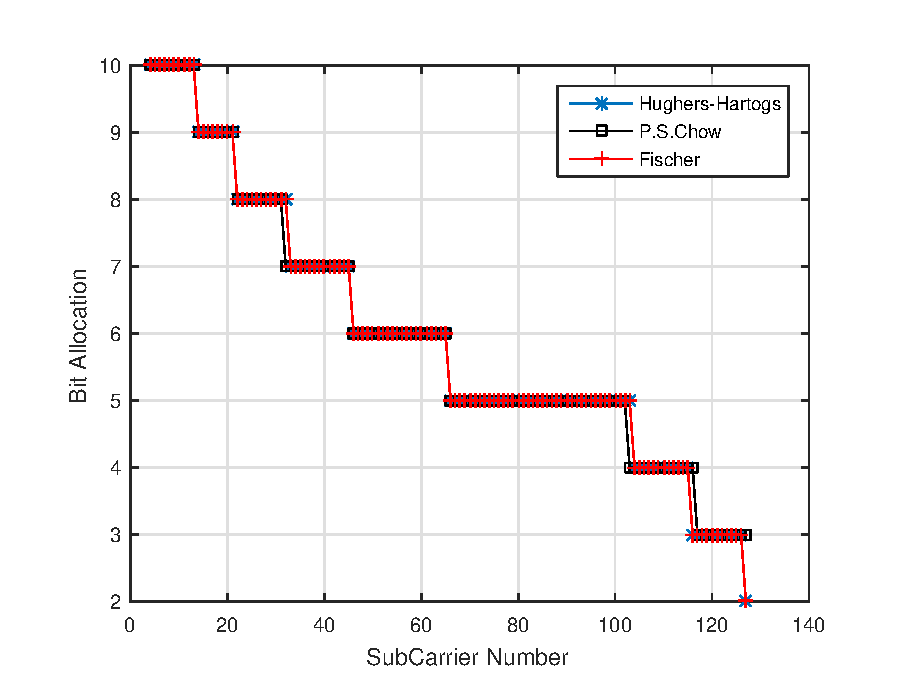
\includegraphics[width=0.8\textwidth]{figures/chapter-4/loadedBit.eps}
\caption{LOS信道下三种算法比特分配结果比较}
\label{fig:loadedBit}
\end{figure}

\begin{figure}[htbp]
\centering
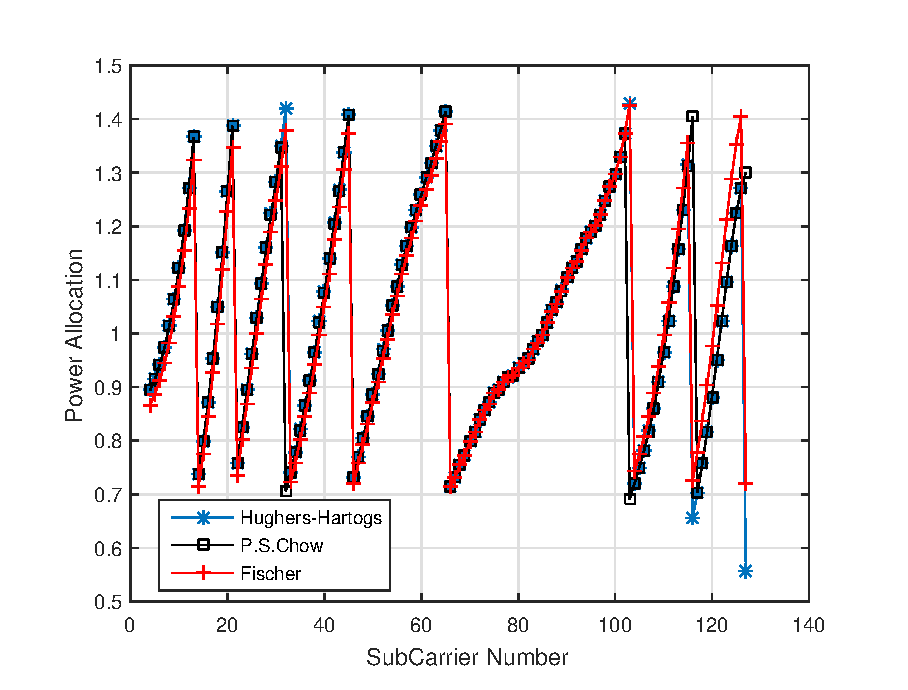
\includegraphics[width=0.8\textwidth]{figures/chapter-4/loadedPower.eps}
\caption{LOS信道下三种算法功率分配结果比较}
\label{fig:loadedPower}
\end{figure}
\section{可见光通信中的自适应方案研究}
前面提到的算法都是具有普适性的,即可以用在任何信道的自适应OFDM系统中,但是我们看到即使Chow算法和Fischer算法相对于Hughes-Hartogs算法进行了简化,但对于实际系统而言复杂度还是偏高的。我们可以充分利用可见光信道的特征,进一步简化比特和功率分配算法。
\subsection{SBLA算法}
从前面的分析及仿真结果可以看到,可见光信道相邻子载波之间存在明显的相关性,特别是LOS信道,信噪比几乎是随频率单调递减的,而不会出现非常明显的起伏,使得相邻子载波之间可支持的调制阶数差别很大。这样的信道条件非常适合用简单分组比特功率分配算法(Simple Blockwise Loading Algorithm,SBLA)\cite{grunheid2000adaptive},该算法的核心思想就是将所有可用的子载波划分为若干个子载波组,每个子载波组使用相同的调制阶数,不同组之间的调制阶数可以不同。这样可以带来两个方面的好处,一是降低了算法复杂度,二是减少了发射端与接收端之间交换的用于协商自适应参数的信令信息。
\begin{table}[ht]
    \caption{各阶QAM调制的门限SNR}
    \label{tab:thresholdSNR}
    \centering
    \begin{tabular}{lllllllllll}
        \toprule
        M-QAM      & 2 &4 &8  &16  &32 &64 &128 &256 &512 &1024 \\
        \midrule
        门限SNR (dB) & 6.9& 10.0&14.5 &16.1 &19.5&22.5&25.4&28.0&31.5&34.5   \\
        \bottomrule
    \end{tabular}
\end{table}

\begin{figure}[htbp]
\centering
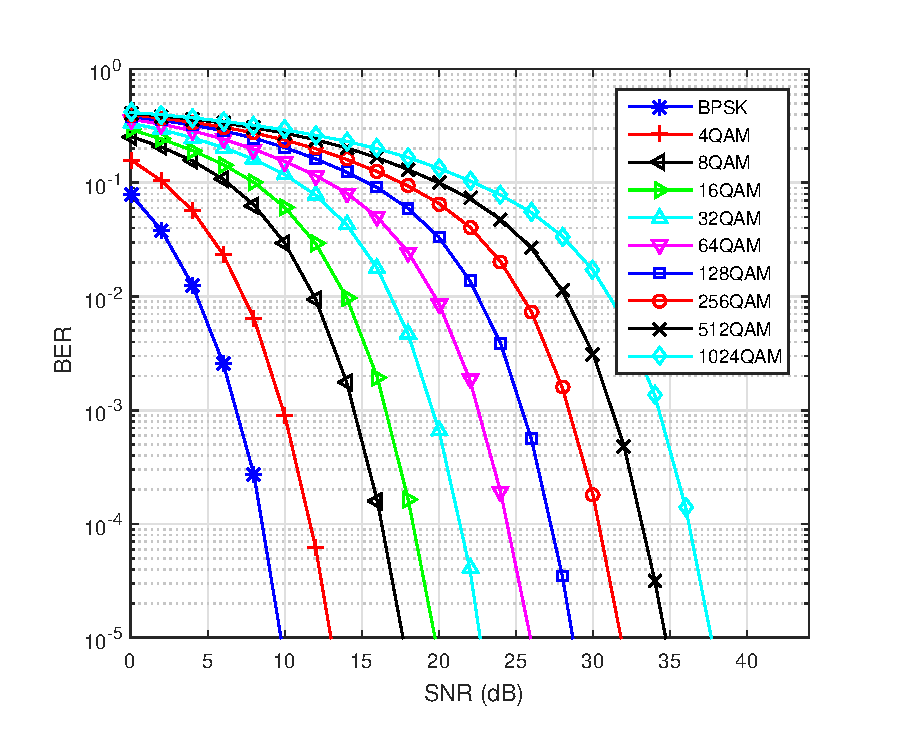
\includegraphics[width=0.8\textwidth]{figures/chapter-4/theoreticalBER.eps}
\caption{AWGN信道下QAM调制的理论BER曲线}
\label{fig:theoreticalBER}
\end{figure}
SBLA算法首先根据目标误比特率和AWGN下QAM各阶调制的BER与SNR之间的关系得到各阶调制的SNR门限,如图\ref{fig:theoreticalBER}所示,我们把目标BER设置为$10^{-3}$,则可以得到如表\ref{tab:thresholdSNR}所示的门限信噪比$SNR_{th}$,有了这组门限值之后可以让每个子载波组的平时信噪比$SNR_{mean}$与这组门限比较,找到满足满足门限的最大调制阶数,这样就可以得到每个子载波组的初始比特分配即总速率,如果总速率$R$等于目标速率速率$R_{target}$则比特分配结束,否则使用类似与Fischer算法步骤6的方法进行调整,下面给出SBLA算法实现的具体步骤:
\begin{description}
\item{\bf{步骤1:}}根据总子载波数量确定分组数$N_B$及每组中包含的子载波数$M$,计算各组的平均信噪比:
\begin{equation}
SNR_{mean}(i) = \frac{1}{M}\sum_{k=1}^M SNR(k), i=1,2,\cdots,N_B
\end{equation}
其中$SNR(k)$表示第i个子载波组中的第k个子载波。
\item{\bf{步骤2:}}根据各子载波组的平均信噪比及信噪比门限,假设第i各子载波组中分配的比特数为$B(i)$,使用条件$SNR_{th}[B(i)]\leq SNR_{mean}(i) < SNR_{th}[B(i)+1]$找到各子载波组的初始比特分配,然后计算并存储平均信噪比与该调制阶数对应的门限信噪比余量$SNR_{diff}(i)$,其定义如下:
\begin{equation}
SNR_{diff}(i) = SNR_{mean}(i) - SNR_{th}[B(i)]
\end{equation}
\item{\bf{步骤3:}}计算初始分配的总速率:
\begin{equation}
R = \sum_{i=1}^{N_B} M \cdot B(i)
\end{equation}
如果$R=R_{target}$,可跳到步骤4,否则进行调整:\\
若 $R>R_{target}$,则找到信噪比余量最小的子载波组,假设其序号为$i^\star$,调整$B(i^\star)=B(i^\star)-1$,$diffSNR(i^\star)=SNR_{mean}-SNR_{th}[B(i^\star)]$,$R=R-M$,继续步骤3直到$R=R_{target}$;\\
如果$R=R_{target}$,可跳到步骤4,否则进行调整:\\
若 $R<R_{target}$,则找到信噪比余量最大的子载波组,假设其序号为$i^\star$,调整$B(i^\star)=B(i^\star)+1$,$diffSNR(i^\star)=SNR_{mean}-SNR_{th}[B(i^\star)]$,$R=R+M$,继续步骤3直到$R=R_{target}$。\\
\item{\bf{步骤4:}}最后根据各个子载波上分配的比特数,按下式计算各子载波上应该分配的功率:
\begin{equation}
\label{equ:calcSLABPower}
p(k) = \frac{P_{total}\cdot \sigma_k^2\cdot 2^{{b}(k)}}{\sum_{i\in \mathrm{I}}\sigma_i^2\cdot 2^{{b}(i)}}
\end{equation}
其中$p(k)$即为所求的第k个子载波上的功率,$b(k)$是表示步骤3中得到的各个子载波上分配比特数,$\sigma_k^2$是Fischer算法中的等效噪声方差,等于实际噪声方差除以信道增益,也就是本算法步骤1中信噪比SNR的倒数。
\end{description}

SBLA算法在初始比特分配和后面的比特调整中都是以子载波组为最小单位的,故在比特分配过程中其算法度是Fischer算法的1/M,M为每组中子载波数,并且在分配过程中不要进行对数运算,而其性能只是略低于Fischer等算法,其仿真结果将在后面给出。
\subsection{减少反馈信息的改进SBLA算法}
SBLA通过每组的方式进行比特分配,降低了这个过程的计算复杂度,并且减少自适应信令信息,除此之外,我们也可以针对可以光信道的特性进一步优化功率分配过程。在前面的SBLA算法中得到了比特分配之后,还是按照类似于Fischer算法对每个子载波进行功率分配,并且接收端要反馈所有子载波的功率值到发射端(假设自适应算法在接收端执行)。但是对于可见光低通信道信道的特点,在每个子载波组中,正常情况下功率分配总是随着频率增加而增加的,因为要想获得低误比特率,要尽量使得每组中各个子载波上的误比特率相等。所以基于这一特点,可以只根据式\ref{equ:calcSLABPower}计算反馈每组子载波中第一个和最后一个子载波的功率,而其他子载波的功率可以使用线性插值得到:
\begin{equation}
p_B(i) = \frac{p_B(M)-p_B(1)}{M-1}*i+p_B(1)\ \ i=2,3,\cdots,M-1
\end{equation}
其中$p_B(i)$表示一个子载波组中第i个子载波的功率,$p_B(l)$、$p_B(M)$是反馈回来的每组中第一个和最后一个子载波功率。根据上式得到各个子载波功率之后再乘以一个系数使得总功率满足发射功率限制即可,我们称这种改进于SLAB的比特功率分配算法为Improved-SLAB算法。

\subsection{仿真结果分析}
图\ref{fig:SBLABERonDiffAlgo}展示了SBLA、Improved-SBLA算法的BER性能。仿真中使用的信道是\ref{subsection:Channel}中的LOS信道,设置子载波总数为128,IFFT点数为256(还有128各共轭对此子载波),并且将0~3及124~127号共8个子载波人为设置为虚拟子载波,不传输数据,所以可用子载波为120个。在SBLA、ImprovedSBLA算法中将这120个子载波分为8组,每组含有15个子载波,目标速率为720 bit/OFDM signal,总功率设为128(与子载波总数相等)。从图\ref{fig:SBLABERonDiffAlgo}可以看到SBLA、Improved-SBLA算法的BER性能相近,并且略劣于Fischer算法,但是较固定比特功率调制和人为挑选的\ref{tab:modOrder}而言,BER还是有较大的提高,这说明了Improved-SBLA算法对SBLA算法的改进是合理的,同时也充分体现了自适应相对于固定调制的优势。
\begin{figure}[htbp]
\centering
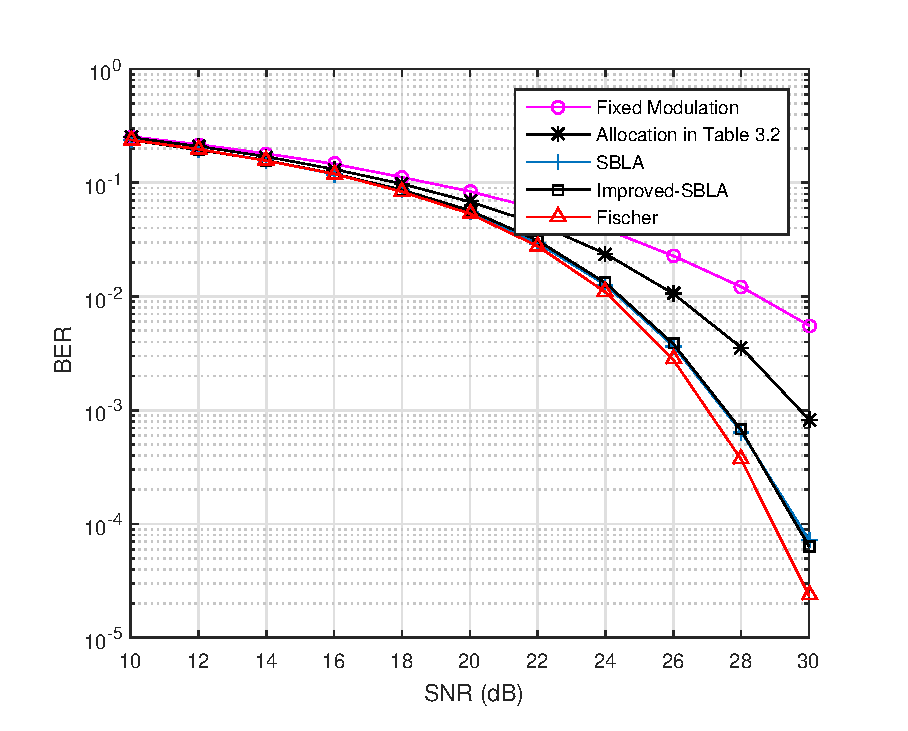
\includegraphics[width=0.8\textwidth]{figures/chapter-4/SBLABERonDiffAlgo.eps}
\caption{SBLA算法及ImprovedSBLA算法BER性能}
\label{fig:SBLABERonDiffAlgo}
\end{figure}

\begin{figure}[htbp]
\centering
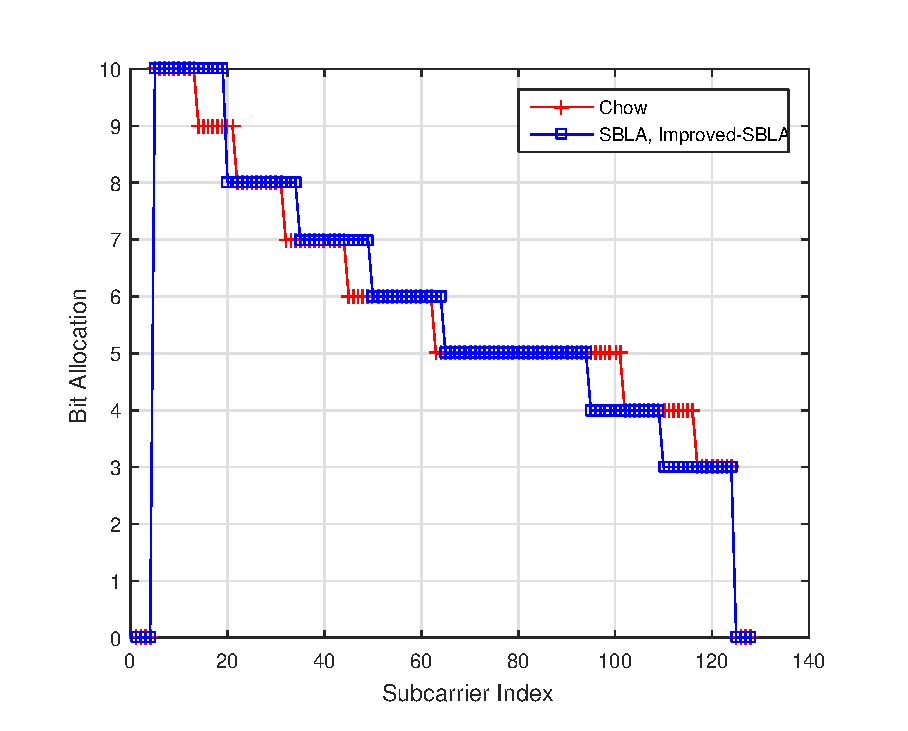
\includegraphics[width=0.8\textwidth]{figures/chapter-4/SBLAloadedBit.eps}
\caption{SBLA算法及ImprovedSBLA算法比特分配}
\label{fig:SBLAloadedBit}
\end{figure}

\begin{figure}[htbp]
\centering
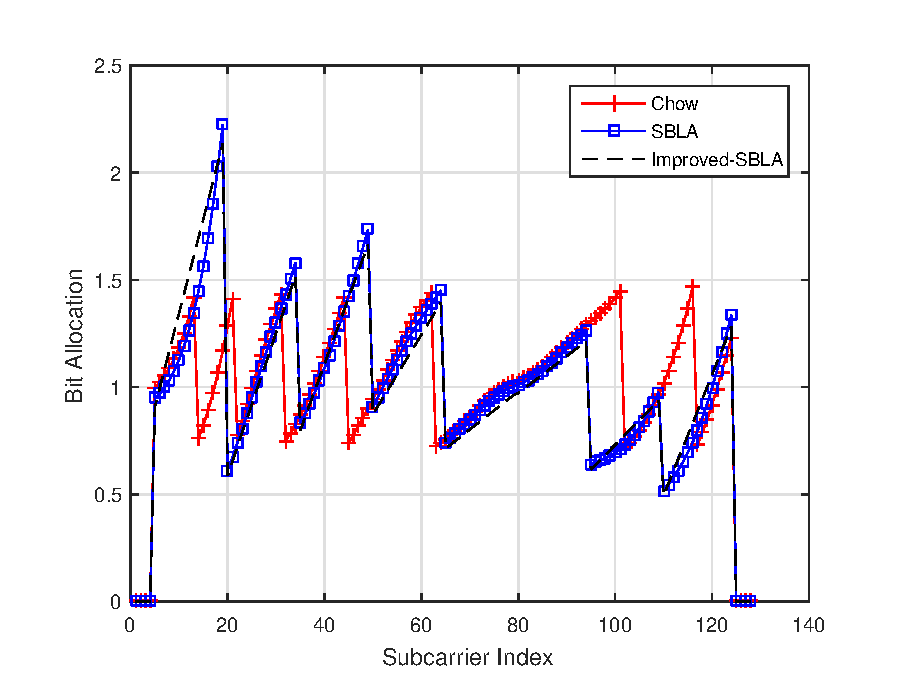
\includegraphics[width=0.8\textwidth]{figures/chapter-4/SBLAloadedPower.eps}
\caption{SBLA算法及ImprovedSBLA算法功率分配}
\label{fig:SBLAloadedPower}
\end{figure}
图\ref{fig:SBLAloadedBit}和图\ref{fig:SBLAloadedPower}给出了设置信噪比为25 dB时在LOS信道下SBLA、Improved-SBLA算法比特和功率在各个子载波上的分配,并且也Fischer算法的结果进行了比较,可以发现SBLA、Improved-SBLA算法因为人为规定了分组,SBLA、Improved-SBLA算法的调制阶数变化只能发生在特定的子载波处,在比特分配上也Fischer算法存在较大的区别,但是还是有一些共性,即低频子载波分配了高阶调制而低频子载波分配低阶调制。从图\ref{fig:SBLAloadedPower}中可以看到SBLA算法在每个子载波组上的是单调递增的,而Improved-SBLA则是利用了这一特性,使用了线性插值来得到功率分配,在图中也可以看出其功率分配在每个子载波组上是呈线性的,并且与SBLA功率分配的结果很接近,这也充分说明了Improved-SBLA算法的合理性。

\section{本章小结}
本章主要介绍了OFDM系统的比特和功率分配算法,研究其在可见光通信中的应用,选出了适合可见光通信的SBLA分配算法,并且在此算法的基础上进行了改进。首先阐述了自适应传输的理论基础—香农信息论和注水定理;然后说明了自适应传输的三种优化准则,即固定目标误比特率和发射功率的最大速率准则(RA)、固定目标误比特率和速率的最小发射功率准则(MA)及固定发射功率和速率的最小误比特率准则(BA),在此基础上介绍了OFDM自适应传输领域三个最经典的算法,分别是在RA和MA准则下最优的Hughes-Hartogs算法、BA准则下Chow算法和Fischer算法,详细说明了这些算法的推导和实现步骤,并且通过仿真比较了它们的性能差异,发现在可见光通信信道下它们在BA准则下BER性能相差不大;最后分析了适合子载波SNR相关性较大的SBLA算法,因为可见光信道本身就是低通的,天然合适SBLA算法的应用,并且进一步利用可见光通信信道特征,提出了适应线性插值来进行功率分配的Improved-SBLA算法,通过仿真发现改进的算法在减少了反馈量及运算复杂度的基础上,BER性能与SBLA相当,说明改进算法是合理可行的。

    \chapter{可见光多波段自适应通信系统硬件设计}
\section{引言}
我们在前面四章介绍了可见光通信的基本原理及关键技术,特别针对自适应传输这个核心重点研究了信道估计及比特功率分配算法,并且针对本课题对应的硬件平台的实际情况进行了必要的仿真,选出了合适的技术方案,如使用低复杂度的LS 算法进行信道估计、使用高精度的EVM方法进行信噪比估计、使用专为可见光通信设计的Improved-SBLA比特功率分配算法得到自适应参数。本章将对可见光通信的硬件系统做一个简要的介绍,还将概述自适应模块的逻辑设计。
\section{硬件平台概述}
本课题对应的硬件演示平台如图\ref{fig:Hardware_Structure}所示,该系统目前已经实现了“编译级”的自适应传输,所谓“编译级”就是代码支持通过改变调制参数然后需要再编译来实现调制的改变,而真正的自适应传输系统因为时间紧迫及反向链路方案尚未确定等因素没有完成。不过本系统已有了自适应传输的雏形了,只是信道估计、计算自适应参数、改变调制等需要离线进行,下面对该系统进行概述。
\begin{figure}[htbp]
\centering
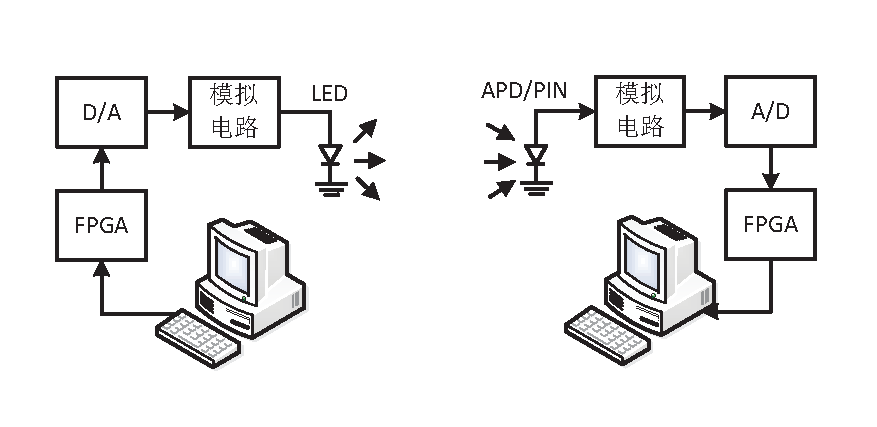
\includegraphics[width=0.8\textwidth]{figures/chapter-5/Hardware_Structure.eps}
\caption{可见光通信硬件平台示意图}
\label{fig:Hardware_Structure}
\end{figure}

首先信源比特通过以太网接口(UDP协议)按帧发送到用于基带处理的FPGA芯片(整个传输过程都是按帧进行的,并且用于同步和信道估计的ZC 序列符号只在帧头处放置,整个帧中所有的OFDM符号都使用这个ZC序列估计出来的信道参数解调),接着在FPGA中完成扰码、信道编码、调制和IFFT等数字处理过程,然后将时域数字信号输入到数字模拟变换器(Digital to Analogue Converter,DAC)变成模拟信号,最后该模拟信号加上偏置电流之后去驱动LED灯,整个发射过程完成。接收端通过PD 接收LED光信号,并将光信号强弱的变化转换成电信号的大小,然后将此模拟电信号送入模拟/数字变换器(Analog to Digital Converter,ADC)中抽样量化为数字信号,再送到接收端基带处理FPGA进行解调、解码和校验等操作,最后输出接收到的帧到接收端计算机。
\subsection{硬件型号及参数简介}
本系统中用于基带处理的FPGA芯片选择美国Xilinx公司生产的Virtex-6,具体型号为XC6VSX315T,基于40 nm工艺,具有高性能、接口丰富等多方面优点。该芯片内部包含49,200个片逻辑单位,每个片逻辑单元中有4个查找表(Look Up Table,LUT)和8个触发器;内置1,344个DSP48数值计算块,每个数值计算块中包含一个$25\times 18$bit 乘法器、一个加法器和一个累加器;同时还有最大存储容量为25,244 kb的嵌入式存储RAM;并且支持千兆网卡\cite{FPGAIntroduciton}。这些资源为我们下面的基带逻辑处理及复杂的LDPC解码运算提供了硬件基础。

DAC选用美国TI公司生成的八通道高速数模转换芯片,型号为DAC3484,其输入数值信号位宽为16 bit,最高支持1 GSps的采样率;ADC芯片同样使用TI公司产品,型号为DAC9643,该芯片支持最高达250 MHz的采样速率,量化精度为14比特。

发射端模拟电路主要包括三部分,功率放大器、直流偏置模块和LED灯。功率放大器选用美国Mini-Circuits公司的ZHL-3A中功率放大器,其3 dB 带宽范围是0.4 MHz ~150 MHz,功率增益25 dB,最大输出功率为 30 dBm;采用的直流偏置模块ZFBT-6GW+同样是Mini-Circuits公司产品,其3 dB带宽范围为0.1 MHz~6 GHz,支持最大偏置电流0.5 A。发光二极管选用美国硅谷光擎(LED Engin)生产的多色混光型发光二极管LED——LZC-03MA07,其发光光谱图如图\ref{fig:LED_LZ4_relativeSputrcalPower}所示。

接收端模拟电路主要由滤光片、光电二极管即放大器。本系统为可见光多波段通信系统,不同的色光用不同的滤波片,分别是蓝光滤光片DTB435、 绿光滤光片DTB530、红光滤光片HB610。光电转换模块选用雪崩型光电二极管(APD),具体型号为C5331-11,生产商为日本滨松公司(Hamamatsu),其3 dB通带为4 KHz~100 MHz,感光区直径1 mm。 接收端低噪声放大器选用美国TI公司生成的OPA847,其带宽增益积为3.9 GHz,输入噪声为$0.85 nV/\sqrt{Hz}$
\subsection{发射端基带处理}
\begin{figure}[htbp]
\centering
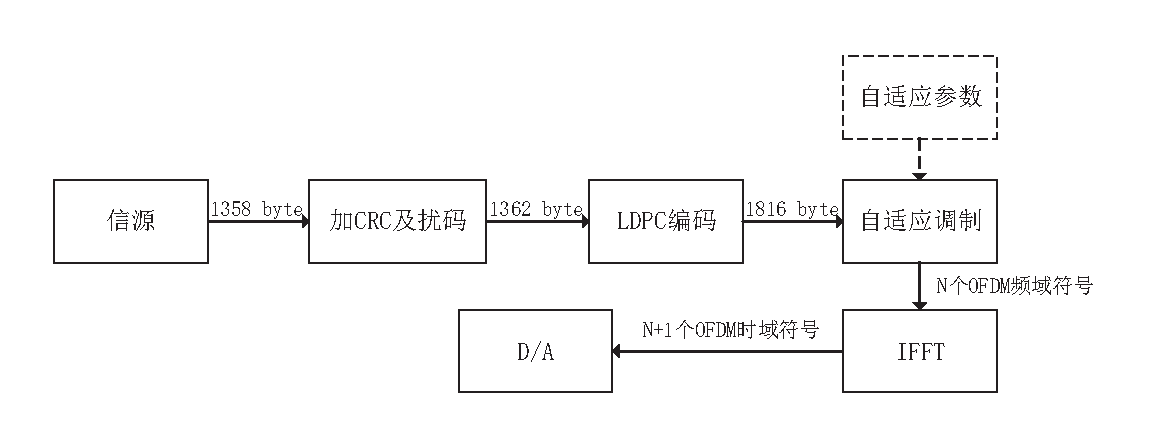
\includegraphics[width=0.9\textwidth]{figures/chapter-5/TransmitterSchematic.eps}
\caption{发射端基带处理原理框图}
\label{fig:TransmitterSchematic}
\end{figure}
发射端FPGA基带处理流程如图\ref{fig:TransmitterSchematic}所示,本演示系统信源帧长定为1358 byte (设置为该值主要是因为本系统主要以视频传输演示为主,而视频帧帧长就是1358 byte),为了系统设计简便起见,当通过以太网接口接到的帧不足1358 byte 时,会自动在后面补零再传输。

基带处理芯片接收到信源帧之后,第一步就是对其加循环冗余校验(Cyclic Redundancy Check,C RC),这里我们使用24 bit 的循环校验码,循环校验比特的生成模块其实就是一个由生成多项式决定的除法电路,输入数据就是被除数,而余数就是我们需要的校验比特,当然为了加快计算速度,本系统CRC使用8位并行计算方法,即不是像真的除法电路那样逐比特地输入,而是一次输入8 比特,整个运算速度提高了8倍。由于篇幅限制,在这里就不对CRC模块再进行过多的展开。得到24 bit(3 byte) 校验位之后添加到原信源数据之后,又因为本系统使用的是输入为1362 byte 的低密度奇偶校验码(Low Density Parity Code,LDPC)作为信道编码,所以1358 byte数据帧加入3 byte 的校验码之后还要补零1 byte。 为了防止过长的连0连1影响系统传输性能,所以还要把加了CRC及补零后的数据进行扰码再送入LDPC编码器。

信道编码是通过在发射数据中增加冗余以便在接收端可以进行信道解码纠错,本系统使用码率为3/4的LDPC码,输入数据长度为$1362\times 8$ bit,输出为14528 bit选择LDPC码的原因是其纠错性能佳,几乎适合所有信道,并且相对于Turbo码而言其解码器实现复杂度要低很多。这里使用的LDPC码的编码矩阵大小为$48\times 227$,所以输入数据位宽要为48 bit,而我们在CRC模块中输出数据位宽为8 bit,所以这里需要位宽变换,可以使用FPGA提供的RAM或先入先出队列(First In First Out,FIFO)数据结构来实现。编码之后的校验比特插在等间隔的插在信息数据中间,因为码率为3/4,每6字节信息数据后插入2个校验字节。

\begin{figure}[htbp]
\centering
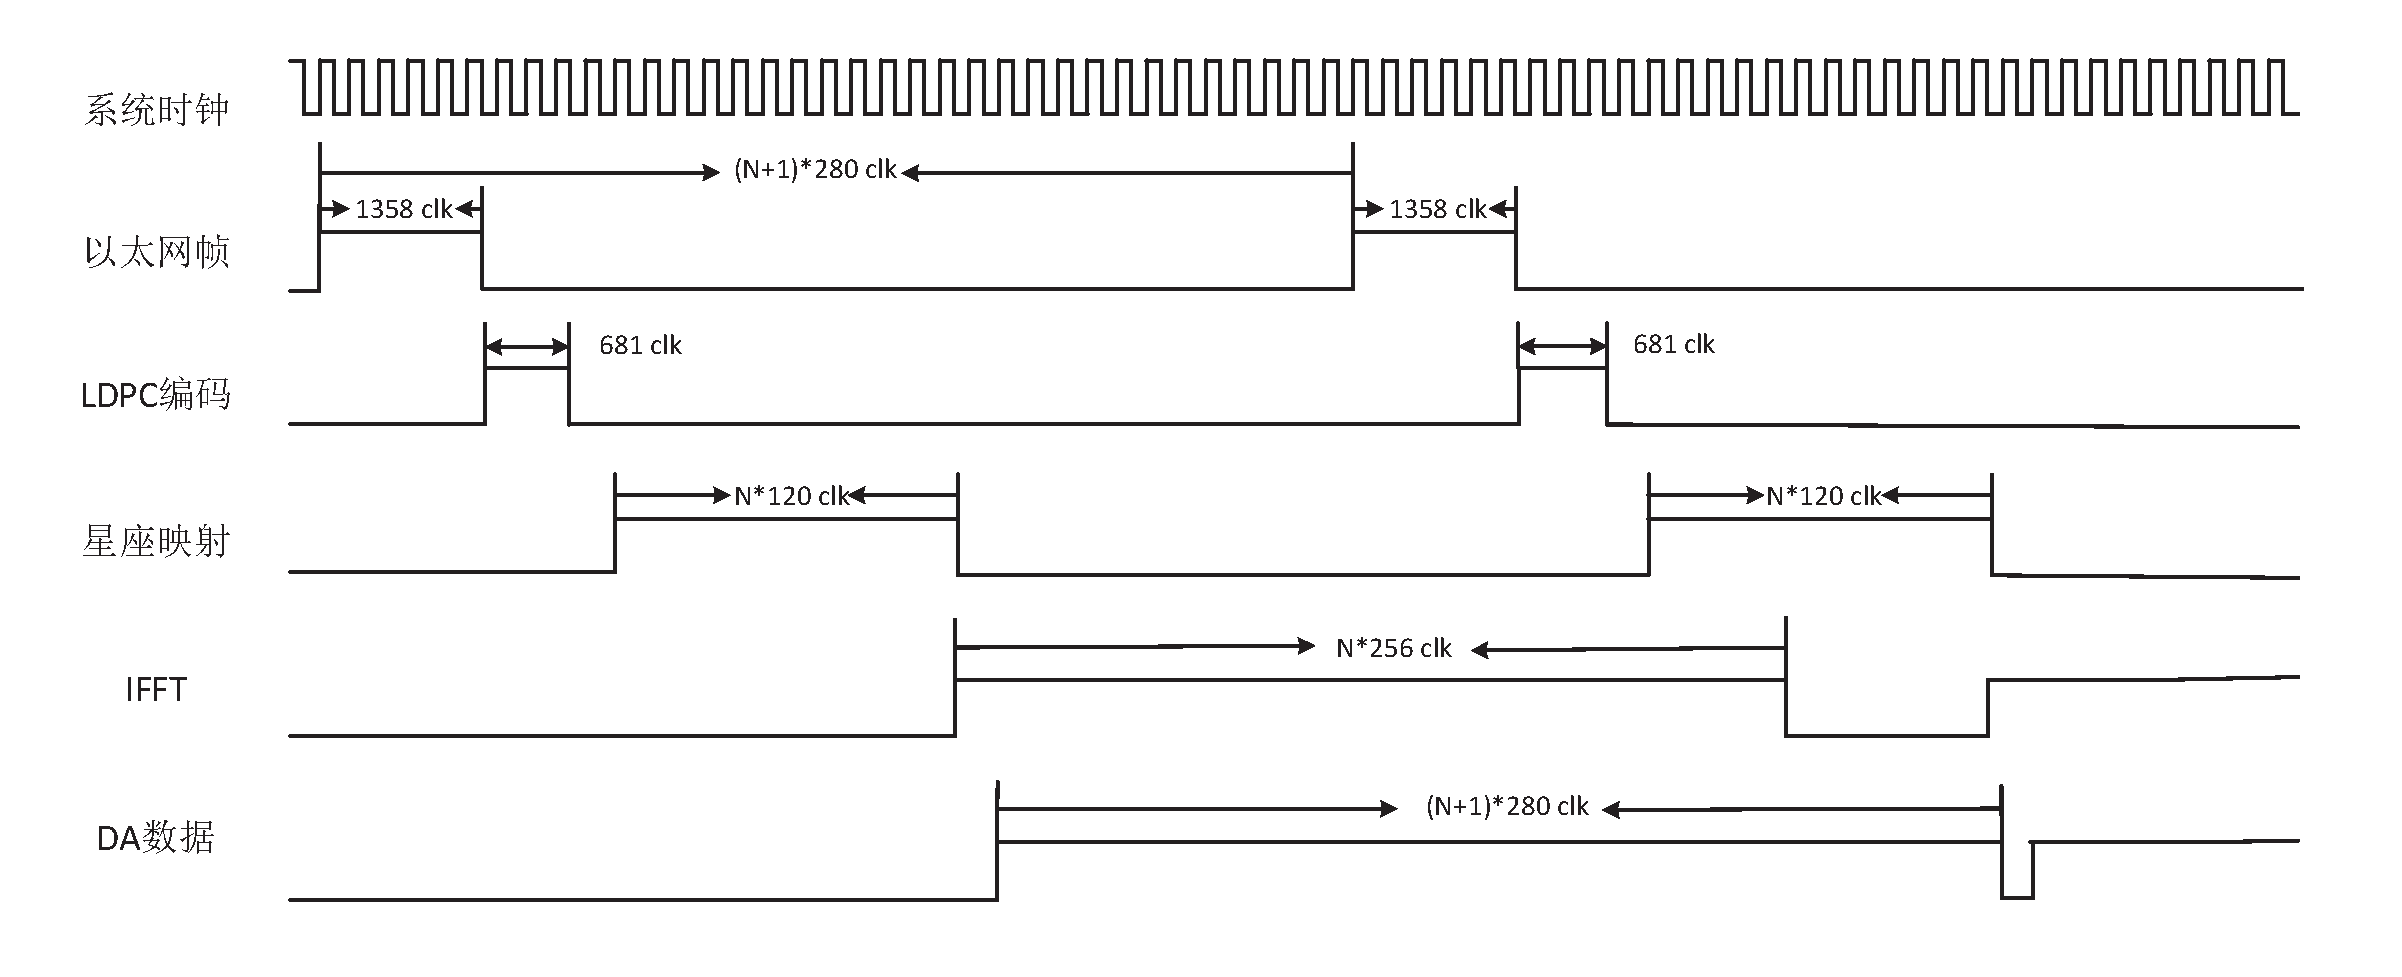
\includegraphics[width=0.9\textwidth]{figures/chapter-5/TimeSchemeTrans.eps}
\caption{发射端基带处理时序图}
\label{fig:TimeSchemeTrans}
\end{figure}
经过编码的帧数据长度变为1816 byte,送入自适应调制模块,其功能是将信息比特分配到OFDM各个子载波上,并映射到星座图中的点,输出OFDM 符号频域数据,这部分属于自适应设计的核心部分,将在下一节详细介绍。

经自适应模块调制后得到N个OFDM符号,N的值也调制的选择有关,假设根据自适应参数每个OFDM符号传输R比特,则有N=$\lceil 14528/\text{R} \rceil$,其中$\lceil \cdot \rceil$表示向上取整运算。为了提高传输速率,要保证所有的操作在一个OFDM帧周期内完成,所以要将将已调制符号交替存入两个RAM中,进行乒乓操作,即如果自适应模块再往其中RAM中写数据,则IFFT模块应该在另一个RAM中读数据去进行IFFT运算,到下一帧时这两个RAM的角色交换。IFFT模块可以使用Xilinx 公司提供的IP核实现,并且可以通过设置自动添加添加循环前缀,非常方便。得到OFDM时域符号之后,在每帧的头部再加上ZC导频序列之后输入到DAC芯片输出,整个发射过程的时序安排如图\ref{fig:TimeSchemeTrans}所示。
\subsection{接收端基带处理}
\begin{figure}[htbp]
\centering
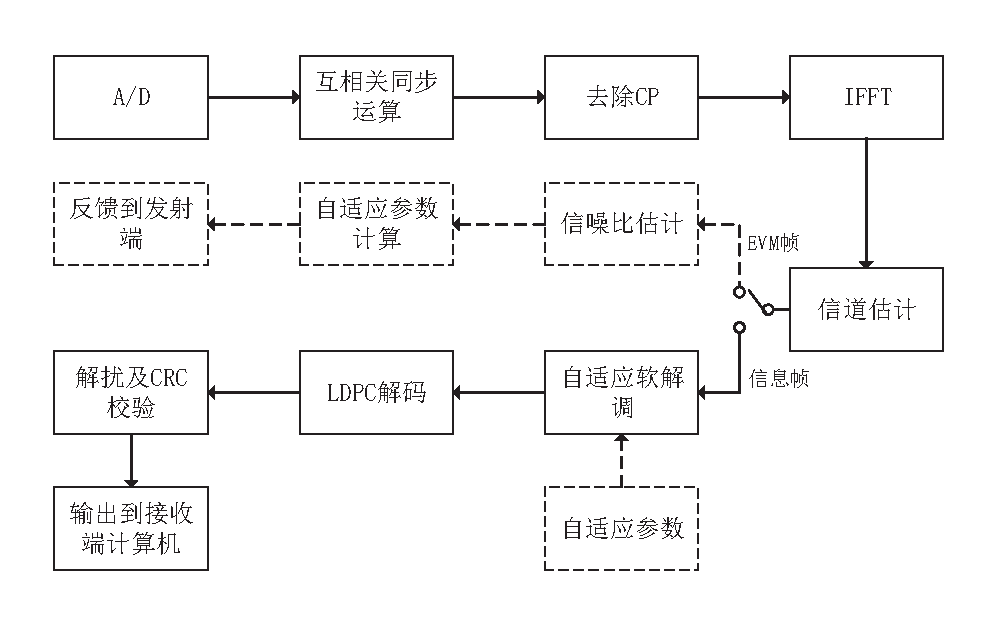
\includegraphics[width=0.9\textwidth]{figures/chapter-5/ReciverSchematic.eps}
\caption{接收端基带处理原理框图}
\label{fig:ReciverSchematic}
\end{figure}
接收端基带处理过程如图\ref{fig:ReciverSchematic}所示,模拟信号经过AD变化之后先与导频时域ZC 序列进行互相关同步运算,互相关结果的峰值所在位置就是导频的开始位置,在现实时为了避免找最大值这样复杂的运算,会通过另外一个模块估计接收信号的功率,从而得到一个互相关阀值,如果互相关结果大于这个阀值就可以认为是同步峰。使用这个特性就能把接收到的信号重新分成一个个OFDM符号,包含1个导频符号和N个信息符号。

因为要使用EVM方法进行信噪比估计,此时需要将用于EVM估计的前导序列放在信息符号发送,我们称这种帧为EVM帧。将这些时域OFDM符号去掉CP,再送入FFT模块,FFT模块输出频域OFDM符号,其中导频符号用于信道估计(使用LS算法),待得到信道估计之后,对信息符号进行单系数均衡,如果是数据帧则送入自适应软解调模块就行解调;如果是EVM帧怎送入信噪比估计模块估计SNR,之后再使用Improved-SBLA算法计算自适应参数,反馈到发射端,这部分也将在下一节展开。
\begin{figure}[htbp]
\centering
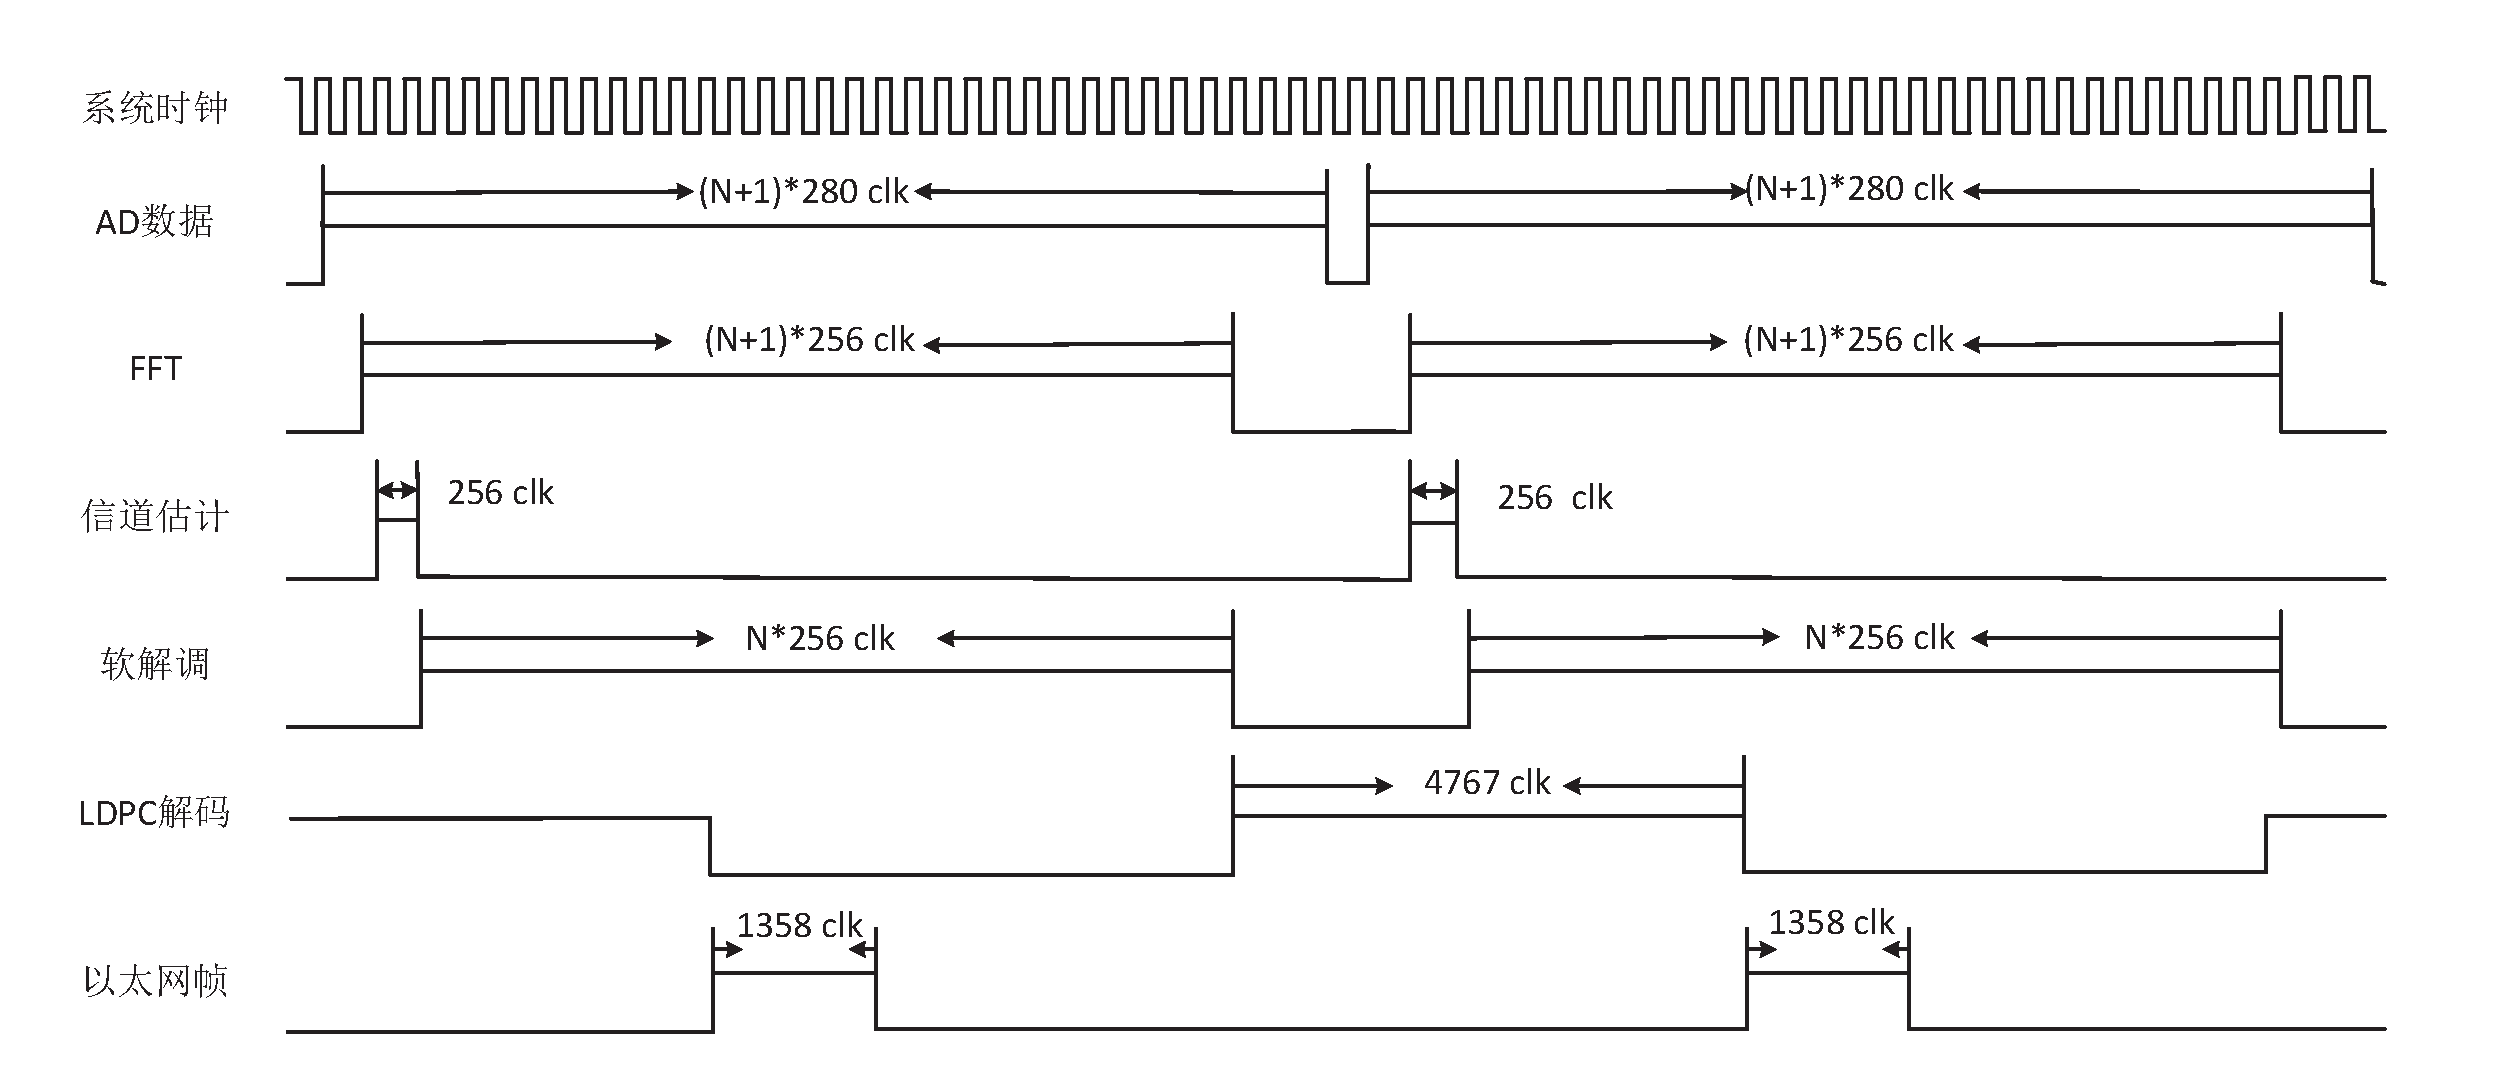
\includegraphics[width=0.9\textwidth]{figures/chapter-5/TimeSchemeRece.eps}
\caption{接收端基带处理时序图}
\label{fig:TransmitterSchematic}
\end{figure}

软解调得到的软件被送入LDPC码解码模块进行解码,软解调的输出位宽因调制阶数不同不同,如使用4QAM调制的子载波软解调输出位宽为16($8\times 2$)bit、16QAM为32 ($8\times 4$)bit、64QAM为48($8\times 6$)bit、256QAM对应为64($8\times 8$)bit,而解码器的输入位宽为$256=8\times 32$ bit,所以这里也存在数据位宽变换的问题,可以先将各阶调制得到的软量存在各自的RAM中,然后统一以64 bit位宽读出到一个FIFO中,再以256 bit位宽读出送入LDPC解码器解码。如接收端基带处理时序图\ref{fig:TransmitterSchematic}所示,解码过程所需要的时间也迭代次数成正比,具体为迭代次数加1再乘以227,本系统设置迭代次数为20,故整个解码过程为4767 clk。 解码器输出位宽为48 bit,经位宽变换为8 bit 之后送入CRC模块进行校验,以统计误帧率,这是系统QoS一个重要的指标。如果通过CRC校验帧正确,则通过以太网接口送入接收端计算机,否则丢弃该帧。


\section{自适应模块方案设计}
上节从硬件参数到基带设计对整个硬件平台进行了简略的介绍,我们已经对整个系统有了一定的认识。在原来的系统上实现自适应传输功能只需就行几个模块的改造,而发射端编码器及之前、接收端译码器及之后等部分都不要变。下面详细介绍这几个涉及到自适应传输的模块。
\subsection{自适应调制模块}
\begin{figure}[htbp]
\centering
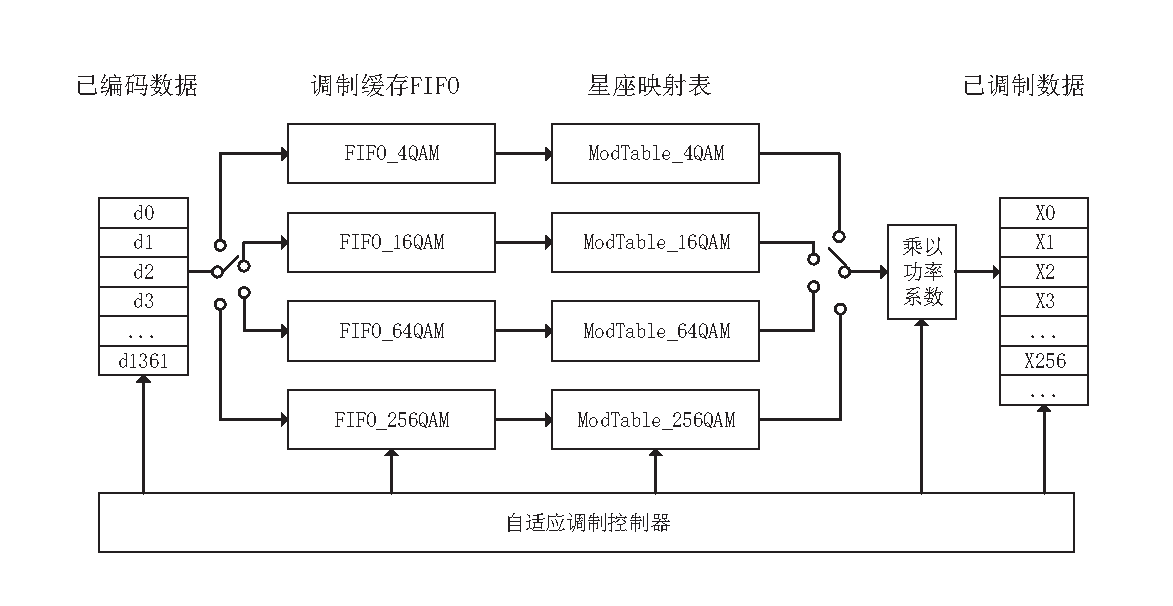
\includegraphics[width=0.9\textwidth]{figures/chapter-5/AdaptiveModulation.eps}
\caption{自适应调制模块示意图}
\label{fig:AdaptiveModulation}
\end{figure}
发射端的自适应调制模块设计如图\ref{fig:AdaptiveModulation}所示,已完成信道编码的数据放在一个位宽为8 bit的RAM中,现在要将这些数据分配到各个子载波上,本系统设计中我们的调制方式限定为4QAM、16QAM、64QAM和256QAM,而每种不同的调制每个符号能够携带的信息比特数也不同,每个M-QAM携带的比特数为$\log_2(M)$。因此先要把已编码的数据根据比特分配表放到不同的FIFO中去,因为FIFO的性质是FIFO 的数据位宽要是输入输出的位宽的倍数,所以用于缓存FIFO的位宽及输入输出位宽如下表所示:
\begin{table}[ht]
    \caption{调制器FIFO参数设置}
    \label{tab:Signle Color Channel Estimation Paramters}
    \centering
    \begin{tabular}{llll}
        \toprule
        FIFO                & 数据位宽  &输入位宽  &输出位宽\\
        \midrule
		FIFO\_4QAM			& 8 bit		&8 bit    & 2 bit  \\
		FIFO\_16QAM			& 8 bit       &8 bit    & 4 bit  \\
		FIFO\_64QAM          & 24 bit       &24 bit    & 6 bit   \\
		FIFO\_64QAM			& 8 bit         &8 bit    & 8 bit  \\
        \bottomrule
    \end{tabular}
\end{table}
所以对于64QAM调制,缓存时需要先拼成24 bit输入,在以6 bit位宽读出。

数据缓存之后,使用查表法进行星座映射。具体是先把各阶QAM调制的已归一化星座点存到不同的ROM中,实部和虚部都按14 bit量化,然后按照各个子载波上的调制阶数,依次从各个FIFO中读出数据,并以此数据为地址,去读该调制下的星座图ROM,输出的数据就是归一化过的星座点,最后再根据功率分配表,乘上功率系数之后存到RAM缓存,同时要注意与之前固定调制不同,这里考虑的功率分配的因素,所以为了接收端简化起见,要在导频ZC序列上各个子载波也要乘以功率系数,这样接收端在解调的时候就不要再专门除以功率系数,会在单系数均衡中处理掉。整个自适应调制器由一个专门的控制器模块来进行时序控制和状态转换。

\subsection{信噪比估计与自适应参数计算}
\begin{figure}[htbp]
\centering
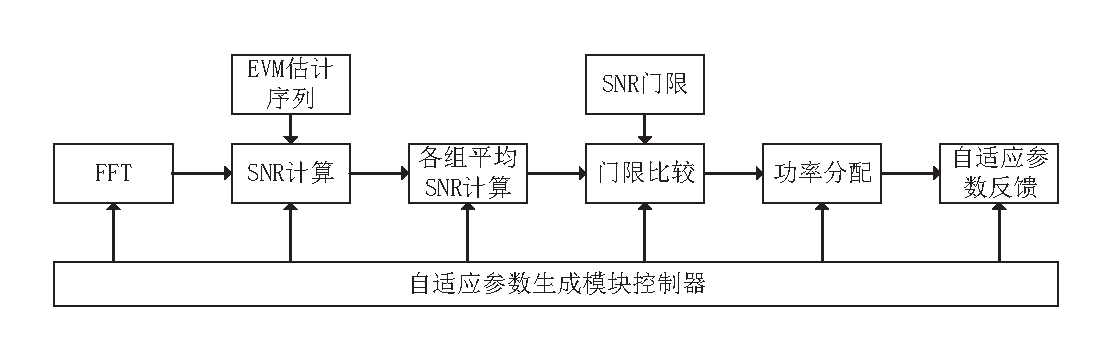
\includegraphics[width=0.9\textwidth]{figures/chapter-5/AdaptiveParameterGenerator.eps}
\caption{自适应参数生成模块示意图}
\label{fig:AdaptiveParameterGenerator}
\end{figure}
信噪比估计及自适应参数计算方案设计如图\ref{fig:AdaptiveParameterGenerator}所示,之前也提过,系统要传输专门的EVM序列来进行SNR估计,这样的帧成为EVM 帧,可以隔固定的时间发送一次,所以处理EVM帧其实就是求当前信道下的自适应参数。

EVM序列频域符号在接收端也是已知的,所以得到已经均衡过的时域符号之后,可以根据公式求得各个子载波上的SNR和噪声方差,每个OFDM符号都能得到一组SNR和噪声方差,可以通过几组值相加求平均的方法来提高估计精度。得到各个子载波上的SNR之后,根据设置的子载波总数和组数,求得每组子载波的平均SNR,然后利用Improved-SBLA 算法来进行比特和功率分配,为了简便起见,保证系统的鲁棒性,我们设置目标BER为$10^{-2}$,同时只按原算法进行初始分配,而不设置目标速率,这样就少了算法后来的循环累加或类减过程。在门限比较时,可以从高门限到低门限比较,当遇到SNR大于某个门限时,就取其对应的调制阶数。得到各个子载波组上分配的比特之后,使用公式求得各个子载波组的第一个子载波和最后一个子载波的功率。将此比特分配和功率分配按照一定的数据格式发送给发射端。
\subsection{自适应软解调模块}
\begin{figure}[htbp]
\centering
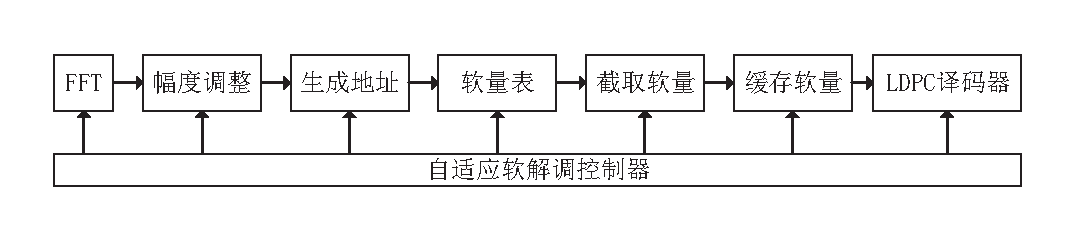
\includegraphics[width=0.9\textwidth]{figures/chapter-5/AdaptiveDemodulation.eps}
\caption{自适应软解调模块示意图}
\label{fig:AdaptiveDemodulation}
\end{figure}
当传输的是数据帧时,自适应软解调按图\ref{fig:AdaptiveDemodulation}所示方案进行软解调,其基本思路是查表法,并且只使用256QAM调制一张表,其他的三种低阶调制通过一些数据变换来时候这张表,按照软量计算理论,实部和虚部分开进行软量计算,并且使用的方法是一样的。下面来介绍具体过程。

经过了单系数均衡后的各个子载波上的频域符号先要进行幅度调制,即乘以其对应的调制阶数的归一化因子,恢复各个调制符号在原始星座图上的幅度,并且要根据调制阶数进行相应的饱和处理,将其限定在对应星座图的范围内,如256-QAM限定在(-16,16)的范围内,64-QAM限定在(-8,8)范围内。然后采用坐标平移的方法让低阶调制能够使用256QAM的软量表,需要对其坐标点搬移到最高阶调制星座图上的合适位置。首先读取当前子载波所用的调制阶数以进行判断,从最低的4QAM移动到16QAM 坐标值减2,16QAM移动到64QAM坐标值减4,以此类推,即$2^k$-QAM向高阶移一阶坐标值减$2^k$/2。因此,对于本设计中各种调制都要移动到256QAM上,256QAM 本身不用移动,64QAM 要减去8,16QAM减去12,4QAM减去14。这样处理完了之后的实部和虚部数据就可以去查软量表了。因为对应的软量是256QAM的,并且软量是按8 bit 量化的,所以从软量表输出的是 32($4\times 8$)bit软量,而低阶调制只是取其中的一部分,如4QAM实部和虚部各传输1 bit,所以取软量表输出最后的8 bit,依次类推就能得到所有的比特软量了。从前所述不难看出,各个OFDM子载波因为调制阶数的不同,所以生成比特软量的速率也不同,所以要把得到的软量按顺序缓存下来,再送入LDPC译码器。

\section{系统展示}
本课题设计的硬件平台如图\ref{fig:Demo}所示,左边的三台计算机用于产生发射信源,T\_Red、T\_Blue和T\_Green发出的数据分别通过多色LED 的红光、蓝光和绿光三个通道发送到接收端;右边三台计算机R\_Red、R\_Blue和R\_Green接收响应色光的数据并显示。

\begin{figure}[htbp]
\centering
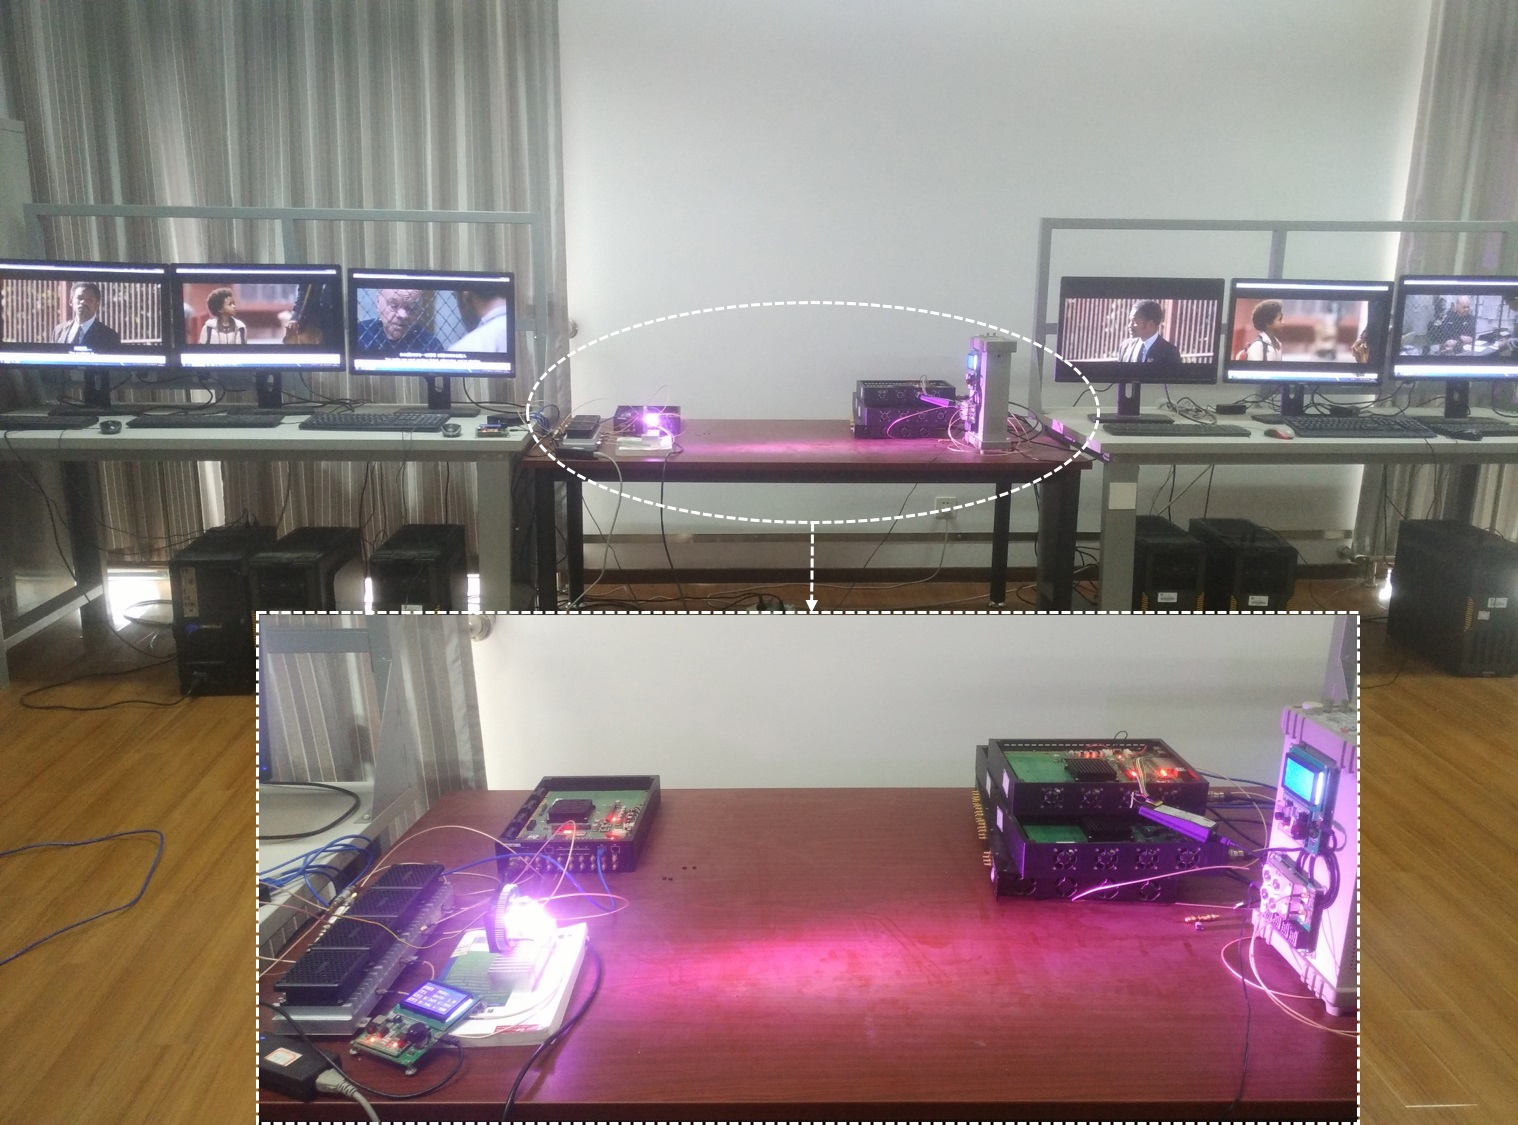
\includegraphics[width=0.9\textwidth]{figures/chapter-5/Demo.jpg}
\caption{硬件平台展示}
\label{fig:Demo}
\end{figure}

表\ref{tab:ExprimentModOrd}给出了我们系统在发射端LED与接收端PD之间的距离为100 cm、采样频率为150 MHz时选择的一组调制方式,其中OFDM子载波总数为128,分为8组,每个子载波组放置16 个子载波,并且将0~3,112~127 号子载波设置为虚拟子载波。可得每路的空间接口速率为291Mbps,总速率873 Mbps。
\begin{table}
\caption{收发机距离100 cm采样频率为150 MHz下各色光的调制及BER}
\label{tab:ExprimentModOrd}
\centering
\begin{tabular}{c|ccccccccc}
\toprule
\diagbox{色光}{子载波组} & 1 & 2 & 3 & 4 & 5 & 6 & 7 & 8 &BER\\
\midrule
Red & 256 & 64 & 64 & 64 & 16 & 16 & 4 & - & 0.0043  \\
Green & 256 & 64 & 64 & 64 & 16 & 16 & 4 & - & 0.0041  \\
Blue & 256 & 64 & 64 & 64 & 16 & 16 & 4 & - & 0.0029  \\
\bottomrule
\end{tabular}
\end{table}


\section{本章小结}
本章在前面几章讲解可见光通信原理及其自适应传输理论的基础上,介绍了本课题对应的硬件平台。首先对整个硬件平台进行了概述,包括各种器件的参数及其选择依据,并且简述了发射端和接收端的基带处理处理过程;然后重点描述了基带处理中与自适应技术密切相关的调制器、自适应参数生成、软解调三个模块;最后展示了整个硬件平台实物图。

%    \chapter{全文总结与展望}
本课题主要讨论了可见光多波段通信领域的自适应传输技术,包括可见光通信的基本原理、信道估计及自适应比特功率分配算法等,最后给出了系统硬件设计方案,下面对全文进行简要的总结并分析该领域之后的研究方向。
\section{论文工作总结}
第一章是绪论。主要介绍了可见光通信的研究背景,包括其应用场景及与传统通信方式相比的优势,同时也对可见光通信在国内外的发展历程进行了概述。

第二章首先可见光通信的基本原理,包括系统模型、信道特征及光电元器件等,本文联系实际情况将可见光通信信道建模为线性信道,然后介绍了电光转换器件LED,详细说明了荧光激发型LED和多色混合型LED的工作原理和特性,还介绍PIN 和APD两类光电转换器件及接收端使用的滤光片。理解这些光电元器件的原理与作用有益于理解整个可见光通信系统。由于OFDM调制技术非常适应光低通信道,在可见光通信中也得到了广泛的使用,所以本章也介绍了光OFDM技术,主要说明了DCO-OFDM和ACO-OFDM的工作原理及区别,在此基础上提出了一种改善ACO-OFDM 系统PAPR 性能的RoC-ACO-OFDM方案,并且在理论和数值仿真的角度论证了该方案的有效性。

第三章主要分析了OFDM信道估计方法的基本原理及其在可见光通信中的应用,首先探讨了OFDM信道估计的常用方法,重点放在基于导频的方法中,系统研究了基于最小二乘法的LS信号估计方法、基于最小均方误差的MMSE方法及其基于MMSE两个改进方法LMMSE和SVD分解方法;然后结合可见光通信系统设计的实例,使用ZC序列作为导频,通过仿真的方法比较了上述方法在可见光信道下的性能,发现虽然LS 信道估计方法在本系统工作点(SNR=25 dB)附近性能稍逊于LMMSE及SVD算法,但是其实现要简便得多,所以在本课题硬件设计中将采用LS进行信道估计;最后讨论了OFDM系统中信噪比的估计方法,分析了基于导频的估计方法和EVM方法,得出了EVM方法虽然需要额外的开销,但是其估计值更加吻合实际系统,推荐在可见光自适应传输系统中使用该方法。

第四章主要介绍了OFDM系统的比特和功率分配算法,研究其在可见光通信中的应用,选出了适合可见光通信的SBLA分配算法,并且在此算法的基础上进行了改进。首先阐述了自适应传输的理论基础—香农信息论和注水定理;然后说明了自适应传输的三种优化准则,即固定目标误比特率和发射功率的最大速率准则(RA)、固定目标误比特率和速率的最小发射功率准则(MA)及固定发射功率和速率的最小误比特率准则(BA),在此基础上介绍了OFDM自适应传输领域三个最经典的算法,分别是在RA和MA准则下最优的Hughes-Hartogs算法、BA准则下Chow算法和Fischer算法,详细说明了这些算法的推导和实现步骤,并且通过仿真比较了它们的性能差异,发现在可见光通信信道下它们在BA准则下BER性能相差不大;最后分析了适合子载波SNR相关性较大的SBLA算法,因为可见光信道本身就是低通的,天然合适SBLA算法的应用,并且进一步利用可见光通信信道特征,提出了适应线性插值来进行功率分配的Improved-SBLA算法,通过仿真发现改进的算法在减少了反馈量就运算复杂度的基础上,BER性能与SBLA相当,说明改进算法是合理可行的。

第五章在前面几章讲解可见光通信原理及其自适应传输理论的基础上,介绍了本课题对应的硬件平台。首先对整个硬件平台进行了概述,包括各种器件的参数及其选择依据,并且简述了发射端和接收端的基带处理处理过程;然后重点描述了基带处理中与自适应技术密切相关的调制器、自适应参数生成、软解调三个模块;最后展示了整个硬件平台实物图。

第六章对全文进行简要的总结并分析该领域之后的研究方向。
\section{展望}
要进行自适应传输,首要条件就是实现双向通信,而目前室内可见光通信的反向链路还没有明确的方案,这个是可见光通信要亟待解决的问题,所以我认为这个领域将引起越来越多研究人员的注意。

另外现在很多研究人员在尝试通过不同的途径来提高可见光通信的传输速率,但针对系统可靠性的研究还不多,特别是在没有直达径下的通信场景,这方面的研究在以后可能也会成为热点。
\end{Main}
% 结束正文

% 参考文献
\bibliography{Reference}

% 附录
%% !Mode:: "TeX:UTF-8"
% 附录

\begin{Appendix}
	\chapter{第一个附录}
	\chapter{第二个附录}
\end{Appendix}
%%%%%%%%%%%%%%%%%%%%论文结尾%%%%%%%%%%%%%%%%%%%%%%%
%\newpage
%\printindex % 索引
%
%% !Mode:: "TeX:UTF-8"

\begin{Resume}
%\fontsize{12pt}{14pt}\selectfont
    \begin{itemize}
        \item 期刊论文
            \begin{itemize}
                \item 第二作者, ``ACO-OFDM-Specified Recoverable Upper Clipping With Efficient Detection for Optical Wireless Communications''.  Photonics Journal, IEEE, 2014, 6(5): 1-17.
                %\item 第一作者, 第二作者, 第三作者, ``Incremental scheduling scheme for indoor visible light communication'', Electronics Letters, Jan. 2015, Accepted.
            \end{itemize}
        \item 专利
            \begin{itemize}
                \item 第二发明人, `` 一种采用削波搬移的低峰均比无线光传输方法'', 申请号:201410206887.X, 2014年5 月.
                %\item ``一种分布式组网光通信系统的灯组协同调度方法'', 申请号:201410191671.0, 2014年6月.
            \end{itemize}
            \begin{itemize}
                \item 第二发明人, `` 一种多色LED可见光通信自适应传输方法'', 申请号:201510019678.9, 2015 年 1月.
                %\item ``一种分布式组网光通信系统的灯组协同调度方法'', 申请号:201410191671.0, 2014年6月.
            \end{itemize}
    \end{itemize}
\end{Resume}
 % 个人简介
%
%% !Mode:: "TeX:UTF-8"
% 致谢

\begin{Acknowledgement}
%\fontsize{12pt}{14pt}\selectfont
时光荏苒,在硕士毕业论文即将完成之际,也意味着紧张、愉快且收获颇丰的研究生生涯就要结束,将要走向人生的下一段旅程,在此,请允许笔者对
曾经指导,教育和帮助过我的老师和同学们略表感情之情。

首先要衷心感谢我的指导老师赵春明教授,在三年的研究生学习中,赵老师的悉心指导让我受益终生。研一时,虽然已上课为主,但是赵老师还是每周
给我们开例会,让我们提前接触科研,为了我之后的发展指明方向;在研究生的第二年,赵老师又亲力亲为指导我们完成科研项目,他丰富的工程经验
帮助我们解决了很多难题,少走了许多弯路;到了研三找工作时,赵老师也为我们的职业发展提供了很多高价值的建议。如果没有赵老师一路来的引导
教育,整个研究生生涯将失色不少。

我也要特别感谢许威老师,许老师负责我研一时的具体指导工作,对我的科研工作进行了启蒙教育。正是许老师严格、细心而又不设限的指导方式让我
很快地进入了科研的节奏,并在研一时就取得了一点点成绩。同时许老师在科研学习中给我充分的自由,当我提出想做些工程方面的工作,许老师也坚
定不移地支持我的想法,让我有机会得到了工程方面的经验。许老师认真、热情、勤奋,与同学们亦师亦友,从他身上我学到了许多。

我还要感谢张华老师,姜明老师,黄鹤老师,梁霄老师在科研生活中给予我的指导和帮助。张华老师除了对我的科研学习上进行指导外,还经常跟我讨
论行业、产业发展的趋势,为我的职业选择提供了宝贵的意见;姜明老师负责实验室很多具体的事物,姜老师的辛勤付出,为了我们营造了一个舒心完
善的科研环境;黄鹤老师精通硬件逻辑编程,教授了我很多工程实现经验;梁霄老师擅长硬件设计,也曾给我很多指导和帮助。课题组的老师们都非常
认真负责,而又平易近人,是他们给了我一个完美的研究生学习经历。

特别感谢实验室的朱清豪,陶于阳,张俊,张立碧,吴宪,刘晶,王佳,邱朗,梁凌轩,官伟,凌欣彤同学,他们让整个实验室在学习过程中充满欢乐,
从他们每个人身上我都学习到了很多。和他们在一起学习和生活的日子,是我研究生生涯中最美好的回忆。感谢实验室成员在项目开发中的互助合作,
正是有大家的帮助才使得本论文得以顺利进行。

另外,我还要特别感谢我的父母和我的哥哥,他们是我最坚强的后盾和最温暖的港湾,我的每一点的进步和成绩都蕴含着他们的心血,也都属于他们。

最后,我还要感谢我的女朋友黄岚,是她伴我成长,给予我学习和生活中的诸多帮助,她也是我不断奋斗的动力源泉。
\begin{flushright}
吴满\\
2016年1月5日\\
\end{flushright}

\end{Acknowledgement}
 % 致谢
%%%%%%%%%%%%%%%%%%%% End of 论文结尾%%%%%%%%%%%%%%%

\end{document}
